% ============================================================
%  The Climate Standoff — Dissertation
%  Compile: pdflatex dissertation.tex  (run twice for refs)
%  Assets resolved via \graphicspath from latex/ directory
% ============================================================
\documentclass[10pt,a4paper]{article}

\usepackage[margin=2.5cm]{geometry}
\usepackage{graphicx}
\usepackage{booktabs}
\usepackage{amsmath,amssymb}
\usepackage{setspace}
\usepackage[hidelinks]{hyperref}
\usepackage{parskip}
\usepackage{microtype}
\usepackage{enumitem}
\usepackage{float}
\usepackage{placeins}  % \FloatBarrier
\usepackage{needspace}
\usepackage{caption}
\captionsetup[figure]{labelformat=empty}
\usepackage{tikz}
\usetikzlibrary{arrows.meta, positioning, calc}
\usepackage{pgfplots}
\pgfplotsset{compat=1.18}

\graphicspath{
  {../results/dissertation/}
  {../results/figures/}
}

\setstretch{1.4}
\setlength{\parindent}{0pt}
\setlength{\parskip}{0.8em}

\widowpenalty=10000
\clubpenalty=10000
\displaywidowpenalty=10000
\interlinepenalty=500

% ── Title helpers ─────────────────────────────────────────
\newcommand{\disssubtitle}[1]{\textit{\Large #1}}
% \bpar prints an inline bold paragraph header. Wrapped in \needspace
% so the header always sits on the same page as the text that follows
% (prevents heading widows at page bottoms), and \nopagebreak prevents
% LaTeX from breaking between the header and the next paragraph.
\newcommand{\bpar}[1]{%
  \par\addvspace{\medskipamount}%
  \needspace{4\baselineskip}%
  \noindent\textbf{#1}\par\nopagebreak[4]%
}

% ── Convenience: bloc colours not needed in text ──────────
\begin{document}

% ============================================================
%  TITLE PAGE
% ============================================================
\begin{titlepage}
\vspace*{0.4cm}
{\noindent\LARGE\textbf{The Climate Standoff:}\\[0.3em]
\large\textit{A Dynamic Game Model of Strategic Tipping in Global Climate Coordination}
\par}

\vspace{0.8cm}

\textbf{Abstract}

\medskip
This paper develops a finite-horizon dynamic Markov game of global climate coordination among four heterogeneous blocs: the United States, China, the European Union, and a developing-economy aggregate. Each five-year period, blocs choose whether to commit to an irreversible low-carbon transition. As the coalition grows, transition costs fall through learning and supply-chain effects while the political and trade costs of remaining outside rise, and collective stabilisation benefits accrue only once a critical participation threshold is crossed. Choice is modelled as probabilistic rather than perfectly optimising, capturing the domestic political friction that prevents governments from behaving as frictionless optimisers, and the game is solved by backward induction.

Calibration proceeds in two stages. Cross-bloc differences in transition costs, climate damages, trade exposure, economic weight, and planning horizons are built directly from World Bank macroeconomic, emissions, and sovereign borrowing data, pinning down how the blocs are positioned relative to each other. The remaining free parameters, which govern how heavily governments weigh upfront costs, future climate damages, the collective payoff from coordination, and the strength with which early adoption pulls later movers in, are recovered by matching the model through simulated method of moments (SMM) to a small set of stylised benchmarks representative of the 2025 climate-policy environment. The fitted baseline is stress-tested through one-at-a-time parameter sweeps and a 1{,}000-draw global sensitivity analysis.

The analysis identifies a sharp ordering among policy channels. Joint planning-horizon improvements in the United States and China are the most efficient single lever: extending both pivotal blocs' horizons together is the only single-instrument intervention that reliably tips a genuinely uncertain baseline into reliable coordination. A robustness exercise across alternative discount-factor orderings, including a US--China flip (Appendix~D), shows this is not US-specific; whichever pivotal bloc starts at the shorter horizon acts as the binding constraint, and joint movement is invariant to which is currently lagging. Reducing transition costs, especially in China, forms a robust second tier and operates as an independent bottleneck that patience alone does not resolve. Learning rates and damage-urgency mechanisms act as amplifiers rather than primary levers.

\vfill
\noindent\textbf{Author:} David Clements\\
\textbf{Supervisor:} Todd R.\ Kaplan\\
\textbf{Academic Year:} 2026\\
\textbf{Word Count:} 10,995
\end{titlepage}

\clearpage
\tableofcontents
\clearpage

% ============================================================
%  1.  INTRODUCTION
% ============================================================
\clearpage
\needspace{12em}
\section{Introduction}

\subsection*{The puzzle: why cooperation sometimes accelerates}

Threshold public goods models explain coordination failure through two interlocking mechanisms:
collective benefits depend on reaching a critical participation mass, and multiple equilibria make that
mass difficult to attain. The literature has produced elegant characterisations of why cooperation stalls. It
has been less successful at explaining why it sometimes accelerates.

The most consequential recent shifts in climate policy were not preceded by formal treaties. The EU's Carbon Border Adjustment Mechanism was designed to support domestic decarbonisation and reduce carbon leakage, phasing in alongside the ETS free-allowance withdrawal as part of the broader Fit for 55 package. The US Inflation Reduction Act reshaped global clean-energy investment through large-scale subsidies, triggering competitive policy responses across Europe and Asia. In both cases, early movers altered the payoff matrix for everyone else; the institutional architecture followed strategic logic rather than producing it.

\subsection*{The strategic environment}

The strategic environment is a multilateral game of chicken. Each bloc would prefer that someone else bear the upfront cost of moving first, but if every bloc holds out the system runs through the climate window and into the catastrophic outcome that everyone wants to avoid. Someone, eventually, has to swerve and adopt; the strategic question is who and when. The players are highly asymmetric. A small number are systemically important enough that their inaction carries disproportionate global consequences, placing them under particular pressure to move first. Others face weak early-mover incentives because short political horizons and high transition costs raise the price of unilateral action. Still others face the sharpest climate vulnerability but the least individual leverage to alter the outcome. The coordination problem is shaped not only by whether blocs eventually cooperate, but by who can afford to delay and whose move most strongly updates others' incentives.

Standard treaty-based models abstract from these features. By treating enforcement pressure, cost trajectories, and threshold progress as exogenous, they cannot account for the timing, escalation, and asymmetry that define modern climate geopolitics.


% ============================================================
%  2.  REVIEW OF LITERATURE
% ============================================================
\clearpage
\needspace{12em}
\section{Review of Literature}

\needspace{12em}
\subsection*{Equilibrium Concepts: Nash to Quantal Response}

The dominant solution concepts in the climate cooperation literature share a common assumption: players
best-respond exactly to the strategies of others. Barrett (1994) uses stage-game Nash equilibrium and
renegotiation-proof repeated-game equilibrium to characterise self-enforcing international environmental
agreements. Harstad (2016) selects Markov perfect equilibrium on the grounds that strategies depending
only on payoff-relevant state variables are both analytically tractable and behaviourally plausible. In
Harstad's dynamic stock-pollution setting, Markov strategies generate a smooth, self-interested incentive
to cut emissions: each player internalises that higher stocks trigger stronger reactions from others,
producing gradual cooperation without requiring external enforcement. The assumption of exact best
response is not incidental to these frameworks. It is load-bearing. Harstad's Markov equilibrium does
produce a cooperation gradient within the dynamic game, but it relies on players computing and
committing to exact best responses to the pollution stock, an assumption that becomes increasingly
demanding when the players are governments subject to domestic political friction.

Carraro and Siniscalco (1993) establish the classical fragility result: stable coalitions under internal and
external stability conditions are typically small, and because participation decisions are discrete, small
parameter changes induce large discontinuous shifts in equilibrium coalition size. The framework moves
abruptly between near-full cooperation and near-complete defection, which limits its usefulness precisely
where the empirical record is most interesting: the margin where marginal incentive changes produce
cascading adoption rather than stasis. While Nash provides a clean benchmark for stability, it offers no gradient for change.

Quantal response equilibrium resolves this by replacing exact best response with probabilistic choice
(McKelvey and Palfrey, 1995). Players choose better options more often, but not always, with choice
probabilities increasing in expected payoffs governed by the rationality parameter $\lambda$. A marginal increase
in adoption costs therefore reduces adoption probability incrementally rather than flipping participation
off entirely. Goeree, Holt, and Palfrey (2003) show that QRE closely tracks observed behaviour across a
wide range of laboratory strategic environments.

Stochastic choice in QRE also has direct political-economy content. Putnam (1988) formalises why governments
cannot behave as frictionless unitary optimisers: international commitments must remain feasible in the
domestic ratification game. Read through that lens, QRE's choice noise admits a structural interpretation as
bureaucratic and ratification friction rather than as purely behavioural error, which makes the framework a
natural fit for an environment in which the players are governments rather than individuals.

QRE ensures smooth incentive changes produce smooth behavioural responses. It does not explain when those responses accumulate into self-reinforcing adoption cascades.

\needspace{12em}
\subsection*{Strategic Tipping and Diffusion Dynamics}

The physical and technological foundations of tipping are reasonably well understood. Way et al.\ (2022)
show that endogenous cost declines through fast learning curves for renewables can shift mitigation
pathways more sharply than most integrated assessment models assume, a finding consistent with the
directed technical change literature establishing that innovation incentives respond to deployment scale in
ways that can generate self-reinforcing cost trajectories (Acemoglu et al., 2012). Farmer et al.\ (2019)
introduce sensitive intervention points in socioeconomic systems, arguing that small, well-targeted
interventions can exploit these amplification mechanisms to trigger cascading low-carbon transitions.
Otto et al.\ (2020) identify specific social subsystems where positive feedback could rapidly compress
emissions trajectories, and Sharpe and Lenton (2021) extend this into a framework of upward-scaling
tipping cascades in which activating one socio-technical tipping point raises the probability of triggering
the next. Milkoreit et al.\ (2018) formalise the social tipping point concept across interdisciplinary
contexts, identifying belief shifts and perceived feasibility as distinct triggers alongside cost and
technology channels.

These contributions capture dynamics observed in real energy transitions. They share a structural
limitation. Adoption decisions are embedded in aggregate diffusion mechanisms, systems feedback
frameworks, or reduced-form cost trajectories rather than arising from explicit strategic interaction
between heterogeneous countries. This matters because the mechanism is difficult to identify. Comin and
Hobijn (2010) document precisely this puzzle in a long historical panel of technology diffusions:
structurally similar countries adopt at systematically different speeds, with institutional and political
factors explaining residual variation that cost differentials alone cannot. Without an explicit strategic
foundation, it is difficult to distinguish whether cascades emerge from cost feedbacks, expectation shifts,
or politically mediated peer effects; the policy implications of each differ sharply.

A second problem compounds the first. Tipping behaviour in formally specified models is often sensitive
to chosen parameter values, making it difficult to distinguish structurally robust dynamics from
calibration artefacts. A finding that holds only at a particular cost trajectory or rationality parameter is not
a finding about tipping. It is a finding about one point in the parameter space.

Taken together, these gaps motivate a framework that endogenises tipping through asymmetric strategic interaction, with a disciplined method for establishing which dynamics survive joint parameter perturbation.

\needspace{12em}
\subsection*{Gaps and Contribution}

Two gaps run through the literature reviewed above. The first is structural. No existing framework jointly
endogenises the three forces the empirical record suggests are co-moving: declining transition costs as the
coalition grows, escalating political pressure on holdouts as the coalition grows around them, and the
asymmetric influence of pivotal blocs whose individual moves shift others' incentives. Coalition models such as
Barrett (1994) and Nordhaus (2015) characterise the participation set at a static club equilibrium---Nordhaus
endogenises the environment through trade penalties on non-members, but the equilibrium is still a
single-shot membership determination rather than a trajectory through time.
Diffusion models such as Grubb et al.\ (2021) capture aggregate cost trajectories but not the strategic
identity of who is adopting and in what order. Neither tradition explains how early adoption by anchor
players reshapes the incentives of holdouts over time.

The second gap is methodological. Kolstad (2007) documents that quantitative results in the IEA literature shift substantially across plausible cost and benefit assumptions, yet few studies distinguish the cross-bloc structure pinned down by observable data from the latent cardinal strength of the payoff channels. Most approaches calibrate to a single benchmark or rely on ad hoc sensitivity checks, making it difficult to tell whether a finding reflects a structural property of the game or a feature of one point in the parameter space.

This paper addresses both gaps. A finite-horizon Markov game with heterogeneous blocs and irreversible adoption characterises behaviour using QRE, allowing smooth comparative statics without the brittleness of Nash-based coalition models.

Calibration is separated into two layers. The ordinal layer is identified from macroeconomic and emissions data. The cardinal layer is recovered by simulated method of moments (McFadden, 1989), matching observable features of the contemporary climate transition: EU leadership, strategic free-riding by major emerging economies, and the delayed onset of self-reinforcing adoption. These produce a single fitted baseline anchored to the 2025 strategic environment.

Marginal sweeps identify which channels matter in isolation. Global sensitivity analysis (Saltelli et al., 2008) stress-tests the rankings by jointly perturbing the full parameter space, separating levers that are locally powerful from those that remain influential once the wider strategic environment moves.

% ============================================================
%  3.  METHODOLOGY
% ============================================================
\clearpage
\needspace{12em}
\section{Methodology}

\needspace{12em}
\subsection{The Model}

\needspace{12em}
\subsubsection*{Players and Structure}

\[
i \in \{\text{US, EU, CN, RoW}\}
\]

Each player represents a geopolitical bloc with distinct economic structures, emissions profiles, and strategic incentives. Using representative blocs is standard in the climate cooperation literature and preserves the asymmetries that shape global outcomes while keeping the model tractable. The United States, European Union, and China together dominate global emissions, renewable manufacturing capacity, and geopolitical influence; the Rest of the World aggregates developing and emerging economies whose individual influence is limited but whose collective climate vulnerability is high. The four blocs are mismatched in a way that makes the cooperation problem hard: the blocs with the most power to act are the least directly threatened by delay, while the bloc most directly threatened has the least power to act on its own.

Time is discrete and finite, indexed by $t = 1, 2, \ldots, T$, where each period represents five years. The horizon is set at $T = 10$ periods, a 50-year window running from the present to roughly the mid-2070s. The finite horizon is not a technical convenience: $T$ represents the point beyond which cumulative emissions lock in irreversible physical damages, consistent with IPCC AR6 and Lenton et al.\ (2019) on biophysical tipping points beyond which further mitigation cannot restore the prior climate state. Beyond $T$ the coordination problem closes rather than continuing in a weakened form, and the value of early coordination derives from the window's closure. In each period, active players simultaneously choose a current-period action $a_{it} \in \{0, 1\}$, where $a_{it} = 1$ denotes adoption. Cumulative adoption status evolves according to the stock-flow law of motion:
\[
G_{i,t+1} = G_{it} + (1 - G_{it})\, a_{it}, \qquad G_{i1} = 0
\]
This makes irreversibility explicit: once $G_{it} = 1$, the term $(1 - G_{it})$ zeroes out any
further action, so the player's status is locked regardless of $a_{it}$. The set of active
players in period $t$ is:
\[
\mathcal{A}_t = \{i : G_{it} = 0\}
\]
Only players in $\mathcal{A}_t$ face a non-trivial adoption decision. Already-adopted players
contribute nothing new to the state.

Each player $i$ is assigned an influence weight $w_i > 0$, normalised so that $\sum_i w_i = 1$.
Influence asymmetry is central to the model's tipping dynamics: early adoption by the US or
China can shift the aggregate state substantially in a single period, while equivalent action
by smaller players cannot.

The payoff-relevant state is the full adoption vector together with elapsed time:
\[
s_t = (t, G_t), \qquad G_t = (G_{1t}, G_{2t}, G_{3t}, G_{4t})
\]
Because costs $c_i(\cdot)$, damages $d_i(\cdot)$, and spillover terms are player-specific,
the identity of who has adopted matters for future incentives: two configurations generating
the same weighted total $W_t$ can imply different active sets and different continuation values.
Cumulative weighted adoption:
\[
W_t \equiv \sum_i w_i G_{it}
\]
is a derived statistic used throughout the payoff functions. Strategies are written as functions
of $(t, W_t)$ for notational clarity where context permits, but the backward induction algorithm
tracks the full adoption vector $G_t$ to correctly compute transition probabilities and identify
active players at each node.

\begin{figure}[htbp]
\centering
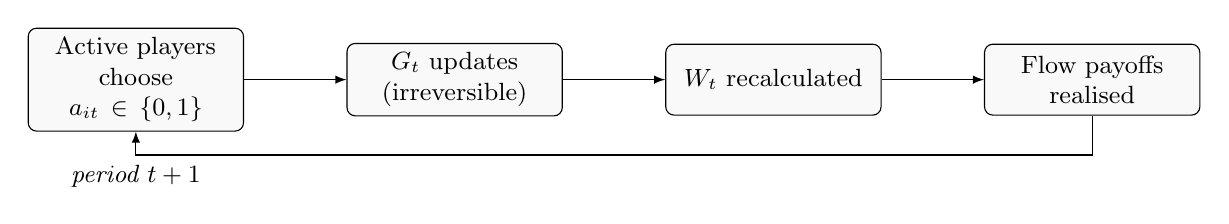
\begin{tikzpicture}[>=latex, node distance=0.5cm and 1.3cm,
  box/.style={draw, rounded corners=3pt, text width=2.5cm, align=center,
              minimum height=0.9cm, font=\small, fill=gray!5}]
\node[box] (a) {Active players\\ choose $a_{it} \in \{0,1\}$};
\node[box, right=of a] (b) {$G_t$ updates\\ (irreversible)};
\node[box, right=of b] (c) {$W_t$ recalculated};
\node[box, right=of c] (d) {Flow payoffs\\ realised};
\draw[->] (a) -- (b);
\draw[->] (b) -- (c);
\draw[->] (c) -- (d);
\draw[->] (d.south) -- ++(0,-0.5) -| node[below, midway, font=\small\itshape]{period $t+1$} (a.south);
\end{tikzpicture}
\caption{Game flow diagram. Each period, active players simultaneously choose whether to adopt.
The adoption vector updates, weighted coalition mass $W_t$ is recalculated, and flow payoffs
are realised before the game advances to the next period.}
\label{fig:game_flow}
\end{figure}

\subsubsection*{Irreversibility of Adoption}

Adoption is modelled as irreversible: once $G_{it} = 1$, the state is locked. This is grounded in the economics of large-scale energy transition, where grid infrastructure, renewable capacity, and retooled supply chains are sunk investments whose abandonment would impose severe losses. Full irreversibility is the limiting case of a costly reversal environment; perfect reversibility would generate a degenerate outcome in which blocs could adopt, observe whether the coalition reaches the threshold, and costlessly undo their commitment. The assumption preserves the commitment risk at the heart of the model.

\begin{figure}[htbp]
\centering
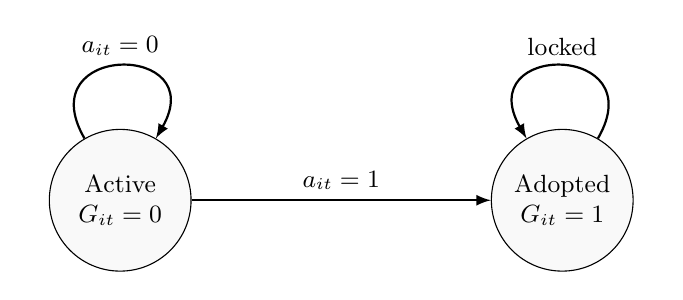
\begin{tikzpicture}[>=latex, node distance=3.8cm,
  st/.style={draw, circle, minimum size=1.8cm, align=center, font=\small, fill=gray!5}]
\node[st] (active) {Active\\ $G_{it}=0$};
\node[st, right=of active] (locked) {Adopted\\ $G_{it}=1$};
\draw[->, thick] (active) -- node[above, font=\small]{$a_{it}=1$} (locked);
\draw[->, thick] (active) to[out=120,in=60,looseness=4]
  node[above, font=\small]{$a_{it}=0$} (active);
\draw[->, thick] (locked) to[out=60,in=120,looseness=4]
  node[above, font=\small]{locked} (locked);
\end{tikzpicture}
\caption{Lock-in and lock-out dynamics. Once a bloc adopts ($G_{it}=1$), its state is
permanently locked. Early movers cannot defect, while holdouts face an escalating cost of
delay as the coalition grows.}
\label{fig:lockin}
\end{figure}

\needspace{12em}
\subsubsection*{Coordination Threshold and Stabilisation}

The economic idea is straightforward: collective benefits are negligible until the coalition
approaches a critical mass, and then activate sharply. A small group of early movers does little
to stabilise the climate on its own, but once the coalition is large enough that it can plausibly
deliver mitigation, the benefit kicks in for everyone. This is captured by a smooth sigmoid
centred at $\theta$ rather than a hard cliff:
\[
S(W) = \frac{1}{1 + \exp(-\eta(W - \theta))}
\]
where $\eta > 0$ controls how sharply the transition activates. Partial coordination delivers partial
benefit, consistent with climate science evidence that incremental mitigation reduces damages
even absent full stabilisation. Marginal returns to coordination are highest near $\theta$,
generating the threshold dynamics central to the model. As $\eta \to \infty$, $S(W)$ approaches
a step function at $\theta$, so the hard threshold case is a limiting special case rather than a
separate model. Both $\theta$ and $\eta$ are varied in the sensitivity analysis.

\begin{figure}[htbp]
\centering
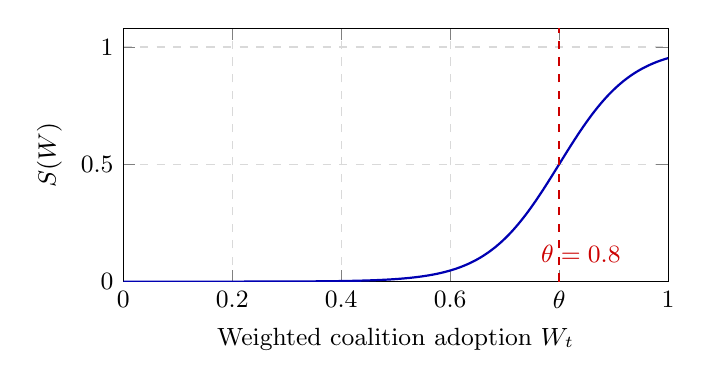
\begin{tikzpicture}
\begin{axis}[
  width=8.5cm, height=4.8cm,
  xlabel={Weighted coalition adoption $W_t$},
  ylabel={$S(W)$},
  xmin=0, xmax=1, ymin=0, ymax=1.08,
  xtick={0,0.2,0.4,0.6,0.8,1.0},
  xticklabels={$0$,$0.2$,$0.4$,$0.6$,$\theta$,$1$},
  ytick={0,0.5,1},
  grid=major, grid style={dashed,gray!30},
  tick label style={font=\small},
  label style={font=\small},
]
\addplot[thick, blue!70!black, domain=0:1, samples=200]
  {1/(1+exp(-15*(x-0.8)))};
\addplot[dashed, red!80!black, thick] coordinates {(0.8,0)(0.8,1.08)};
\node[font=\small, text=red!80!black] at (axis cs:0.84,0.12) {$\theta=0.8$};
\end{axis}
\end{tikzpicture}
\caption{Stabilisation benefit as a function of weighted coalition adoption. The sigmoid $S(W)$
activates sharply as $W_t$ crosses the coordination threshold $\theta = 0.8$ under the baseline
steepness $\eta = 15$; the dashed line marks where collective action tips from partial to
near-full stabilisation.}
\label{fig:state_viz}
\end{figure}

This threshold structure generates the model's core strategic tension. Early adoption imposes immediate transition costs but delivers negligible benefit: $S(W)$ is flat well below $\theta$, so a lone early mover shifts their own cost burden without materially accelerating stabilisation. The collective benefit only becomes substantial as the coalition approaches critical mass. Patience, attainability beliefs, and the composition of the early coalition are therefore the dominant strategic variables.

\needspace{12em}
\subsubsection*{Flow Payoffs}

All flow payoffs in period $t$ are evaluated at $W_t$, the cumulative adoption state at the
\textit{start} of the period, before current actions are realised. Under simultaneous choice,
no player observes others' period-$t$ decisions when choosing. Adopters incur the one-off
transition cost in the period of adoption; any learning spillover from their own action enters
only future periods via $W_{t+1}$.

\bpar{Transition Costs:}
Adoption involves a one-off cost paid in the period of adoption that declines as the coalition
grows:
\[
c_i(W_t) = c_i^0\,(1 - \gamma\, W_t)
\]
The parameter $c_i^0$ captures each bloc's baseline transition burden before any coalition has
formed, and the learning rate $\gamma \in [0,1]$ governs how quickly costs fall as adoption
spreads. Falling costs reflect technology transfer, supply chain deepening, and learning-by-doing
as more producers move down the deployment curve.

\bpar{Political Pressure:}
Active players who delay face political pressure that grows linearly with coalition size:
\[
p_i \cdot W_t
\]
The pressure sensitivity $p_i$ reflects each bloc's exposure to trade restrictions, diplomatic
isolation, and reputational costs from non-cooperation. The linear specification implies that
holding out becomes proportionally more costly as the coalition grows around the holdout.

\bpar{Climate Damages:}
Countries face damages that escalate over time and diminish as coordination approaches the
threshold:
\[
d_i(t, W_t) = d_i^0 \cdot (1 + \kappa t) \cdot (1 - S(W_t))
\]
The baseline vulnerability $d_i^0$ captures structural economic exposure to climate risk. The
temporal escalation term $(1 + \kappa t)$ introduces a deadline effect: the longer coordination
takes, the worse the consequences. Damages are non-excludable: only the collective level of
adoption $W_t$ matters, not any individual player's action.

\bpar{Stabilisation Benefit:}
All players receive a per-period benefit as adoption approaches the threshold:
\[
b \cdot S(W_t)
\]
The benefit is non-excludable: even players who have not adopted receive it as the world
stabilises, preserving the free-rider incentive throughout the game. The scaling parameter $b$
captures the aggregate economic value governments place on avoided climate damages from
successful global stabilisation, the collective payoff from coordination success that no single
bloc can secure alone. Unlike transition costs and climate damages, which are anchored to
observable data in Layer~1, $b$ is not directly observable from national accounts and is
recovered by SMM alongside the other cardinal weights.

\bpar{Combined Flow Payoffs:}
The state-contingent component received by all players regardless of action:
\[
r_i(t, W_t) = -d_i(t, W_t) + b \cdot S(W_t)
\]
For active players ($i \in \mathcal{A}_t$), the action-specific payoffs are:
\begin{align*}
r_i^A(t, W_t) &= -c_i(W_t) + r_i(t, W_t) \\
r_i^D(t, W_t) &= -p_i\, W_t + r_i(t, W_t)
\end{align*}
For already-adopted players ($i \notin \mathcal{A}_t$), the transition cost has been paid in
full and their period payoff is simply $r_i(t, W_t)$.

\bpar{Discount Factors:}
Each player $i$ is assigned a discount factor $\delta_i \in (0,1)$. A payoff received in
period $t+1$ is worth $\delta_i$ times the same payoff in period $t$. Higher values reflect
greater patience: a bloc that values future payoffs highly has stronger incentives to invest
in early coordination. Bloc-specific values are discussed in the Calibration section.

These two parameters capture conceptually distinct sources of strategic inertia and should
not be conflated. $\delta_i$ governs the length of a bloc's effective planning horizon:
how far into the future its institutions credibly weight consequences. $\lambda$ governs the
precision of strategic choice around that horizon: the degree of political noise, bureaucratic
friction, and domestic constraint that prevents even a patient bloc from acting as a
frictionless optimiser. A bloc can have a long planning horizon but high political noise
(high $\delta$, low $\lambda$), or a short horizon executed with institutional precision
(low $\delta$, high $\lambda$). The two parameters do different things and are identified
through different variation in the analysis.

\bpar{Cost--Pressure Identification and the Composite Spillover Channel:}
The transition-cost and political-pressure mechanisms are conceptually distinct economic
channels but both intensify with the same state variable $W_t$: falling costs pull potential
adopters in, rising pressure pushes holdouts in, and an acceleration along any equilibrium
adoption path is consistent with either channel doing the work, or any mixture of them. This
matters for the calibration exercise introduced in the next section, because no moment
constructed from adoption trajectories can cleanly separate the cardinal weight of cost learning
from that of political pressure. The calibration handles this by collapsing the two mechanisms
into a single composite \textit{adoption spillover channel} carrying one cardinal weight, with
an internal mixing parameter $\phi \in [0,1]$ controlling the split:
\begin{align*}
c_i(W_t) &= c_i^0 - \tilde{c}_i\,(1 - \phi)\,\gamma\,W_t \\
\text{pressure}_i(W_t) &= \phi\, p_i\, W_t
\end{align*}
Here $\tilde{c}_i$ is the bloc's cost-learning spillover magnitude, scaled separately from the
baseline cost level $c_i^0$ so that the calibration can recover the level and the spillover
strength as distinct parameters. $\phi$ is held fixed at $0.5$ during estimation and swept across
its full range in the sensitivity analysis (Appendix~B), which establishes that the recovered
weights are stable across the identifiable region. Intuitively, the cost-learning side is the
\textit{carrot} (technology transfer, concessional finance, supply-chain cooperation); the
pressure side is the \textit{stick} (trade conditionality, carbon border adjustments, diplomatic
exposure). Both push toward more adoption but operate through conceptually distinct policy
instruments. Whether one dominates the other in shaping coordination outcomes is an empirical
question the GSA returns to.

\needspace{12em}
\subsubsection*{Recursive Value Structure}

Each bloc is forward-looking. When deciding whether to adopt or wait in a given period, it weighs
the immediate payoff of each choice against the discounted value of all future periods, taking
others' likely behaviour into account. The two action-specific values are written as $Q_i^A$
(adopt) and $Q_i^D$ (delay), each adding the current flow payoff to the discounted expected
continuation value:
\begin{align*}
Q_i^A(s_t) &= r_i^A(t, W_t) + \delta_i\, \mathbb{E}[V_i(s_{t+1}) \mid a_{it} = 1] \\
Q_i^D(s_t) &= r_i^D(t, W_t) + \delta_i\, \mathbb{E}[V_i(s_{t+1}) \mid a_{it} = 0]
\end{align*}
The conditioning on $a_{it}$ matters: player $i$'s own action shifts $W_{t+1}$ by $w_i$ if
they adopt, altering the distribution over future states and the expected continuation value
of each choice. The recursion ends with the terminal condition $V_i(T+1, \cdot) = 0$.

The continuation value $V_i$ averages over the bloc's own future choice. Because behaviour is
noisy rather than deterministic, this average takes a smoothed form:
\[
V_i(s_t) = \frac{1}{\lambda} \log\!\left(e^{\lambda Q_i^A} + e^{\lambda Q_i^D}\right)
\]
This expression is the standard logit value function. It is the expected value when each bloc's
choice is subject to small unobserved payoff shocks with precision $\lambda$. Specifically, if the
shock attached to each action is drawn independently from a Type I extreme value (Gumbel)
distribution with scale parameter $1/\lambda$, the expectation $\mathbb{E}[\max\{Q_i^A + \varepsilon^A,\,
Q_i^D + \varepsilon^D\}]$ is exactly the log-sum-exp form above. This is the same result that
delivers the multinomial logit in discrete choice (McFadden, 1973) and is what makes the
smoothing functional form natural rather than ad hoc. Higher $\lambda$ means tighter, more
deterministic behaviour: as $\lambda \to \infty$, $V_i(s_t)$ collapses to the maximum of $Q_i^A$
and $Q_i^D$, recovering the standard rational-agent Bellman equation.

For already-adopted players ($i \notin \mathcal{A}_t$):
\[
V_i(s_t) = r_i(t, W_t) + \delta_i\, \mathbb{E}[V_i(s_{t+1})]
\]
Future utility continues to depend on the $W$ trajectory driven by the remaining active players.

\needspace{12em}
\subsubsection*{Equilibrium}

Equilibrium adoption probabilities are defined over active players and follow the logit QRE
formula. For $i \in \mathcal{A}_t$:
\[
\sigma_i(s_t) = \frac{\exp\{\lambda Q_i^A\}}{\exp\{\lambda Q_i^A\} + \exp\{\lambda Q_i^D\}}
\]
For $i \notin \mathcal{A}_t$, $\sigma_i(s_t) = 0$ by the irreversibility constraint.
Equilibrium is a fixed point in the mapping from beliefs over opponents' actions into optimal
logit response probabilities:
\[
\sigma^* = \mathrm{QRE}(Q(\sigma^*))
\]
No player wishes to revise their strategy given others' strategies, and others' strategies are
consistent with those beliefs. The game is solved by backward induction from period $T$. At
each state, fixed-point iteration finds the self-confirming probability vector.

\subsubsection*{Solution Method}

The finite horizon and irreversibility together make backward induction the natural and exact
solution method. The finite horizon provides a well-defined terminal condition $V_i(T+1,\cdot)=0$
from which the recursion unwinds cleanly. Irreversibility ensures the state space is
monotonically non-decreasing: once $G_{it}=1$, the player never returns to $\mathcal{A}_t$.
This bounds the number of distinct adoption configurations at each period to at most $2^4 = 16$,
making exhaustive enumeration computationally trivial. The backward induction algorithm stores
$\sigma_i(t, G_t)$ and $V_i(t, G_t)$ at each node, referenced by earlier periods without
recomputation. The full dynamic game is solved exactly in a single backward pass through the
game tree.

\needspace{12em}
\subsubsection*{State Transitions}

The adoption vector evolves according to:
\[
G_{i,t+1} = G_{it} + (1 - G_{it})\, a_{it} \qquad \forall\, i
\]
from which cumulative weighted adoption is derived:
\[
W_{t+1} = \sum_i w_i\, G_{i,t+1}
\]
For a given action profile $(a_{jt})_{j \in \mathcal{A}_t}$, the probability of moving from
$G_t$ to $G_{t+1}$ is:
\[
\Pr(G_{t+1} \mid G_t, \sigma) =
  \prod_{j \in \mathcal{A}_t} \sigma_j(s_t)^{a_{jt}} \left(1 - \sigma_j(s_t)\right)^{1-a_{jt}}
\]
Each active player's decision enters as an independent Bernoulli trial. Expected continuation
values sum over all reachable $G_{t+1}$:
\[
\mathbb{E}[V_i(s_{t+1}) \mid a_{it}] =
  \sum_{G_{t+1}} \Pr(G_{t+1} \mid G_t, \sigma, a_{it}) \cdot V_i(t+1, G_{t+1})
\]

% ============================================================
%  3B.  DATA AND CALIBRATION  (subsection of Methodology)
% ============================================================
\clearpage
\needspace{12em}
\subsection{Data and Calibration}

Implementing the model requires assigning numerical values to all parameters. Some can be disciplined
directly by observable data. Others cannot. The calibration strategy addresses this by separating the
problem into two layers, each with a distinct identification logic.

The first layer fixes ordinal structure: the relative positioning of blocs within each parameter channel. Cross-bloc rankings in transition costs, climate damages, and systemic influence can be inferred from data. The EU's position is identified from carbon intensity, trade openness, and deployment history; the SMM moments then target the magnitude of the EU--peer gap, not its existence. World Bank (2026) development indicators, national emissions inventories, and bilateral trade statistics provide the evidence base. This layer is held fixed throughout: perturbing it would mean contradicting the observable record.

The second layer recovers cardinal scaling: the relative importance governments place on transition costs, adoption spillovers, climate damages, and coordination benefits is not observable from macroeconomic data (Nordhaus, 2007) and is estimated using simulated method of moments (McFadden, 1989).

Ordinal structure is data-identified. Cardinal scaling is structurally estimated. The sensitivity analysis is conducted around this fitted baseline, which is what allows the distinction between locally powerful levers and structurally robust ones to carry empirical weight.

% ---- 4.1 Layer 1: Ordinal Structure -------------------------
\needspace{12em}
\subsubsection{Layer 1: Ordinal Structure}

Each per-player parameter is constructed from bloc-level World Bank (2026) data through a structural transformation anchored to the EU as the reference bloc, so that a single scaling $\alpha$ sets the EU's level and the other blocs follow data-implied ratios. The EU is used as the numeraire because its long continuous record of climate legislation and ETS operation makes its bloc-level values the best-anchored data point; this is a normalisation convention only, and the EU--US gap that appears later as a calibration moment is a moment about magnitude rather than about which bloc is the anchor, so no circularity is introduced.

\bpar{Transition costs} are derived from the carbon intensity of GDP, adjusted for development. Raw intensity is misleading for less developed economies, where low values often reflect limited industrialisation rather than clean infrastructure. A development-gated interpolation blends each bloc's observed intensity with a global baseline, weighted by GDP per capita relative to the richest bloc. An affordability penalty is then applied (elasticity $\epsilon = 0.3$) to capture the higher cost of capital for renewable deployment in developing economies (Ameli et al., 2021). Together these adjustments ensure the ordinal cost structure reflects genuine transition burdens.

\bpar{Climate damages} are proxied by the share of agriculture, forestry, and fishing in GDP, capturing structural economic exposure to climate risk. Burke et al.\ (2015) document that agricultural productivity losses account for the largest share of measurable climate damages across income levels; the proxy is preferred over composite indices like ND-GAIN for its direct observability and cross-bloc consistency.

\bpar{Political pressure} is proxied by trade openness (trade as a share of GDP). A more trade-dependent economy has more to lose from non-cooperation: carbon border adjustments, climate-linked conditionality, and diplomatic friction all arrive through trade relationships.

\bpar{Influence weights} are a GDP-weighted combination of emissions share and GDP share (0.30/0.70). Emissions share captures necessity for any effective coalition; GDP share captures the economic channels through which adoption influence operates. The 70/30 weighting is varied in the robustness checks reported in the appendix.

\bpar{Special Note on Player Discount Rates:}
Discount factors $\delta_i$ reflect the effective length of each bloc's credible planning horizon: how
far into the future its institutions act as if they weight future payoffs (Nordhaus, 2007). They are
deliberately descriptive rather than prescriptive.

The EU receives $\delta_{EU} = 0.85$ (implied annual rate $\approx 3.3\%$), reflecting the legal
bindingness of the European Climate Law and over two decades of continuous ETS operation. China is
assigned $\delta_{CN} = 0.80$ ($\approx 4.6\%$), where centralised governance supports continuity
through the five-year plan system but growth constraints shorten the effective horizon. The United
States receives $\delta_{US} = 0.75$ ($\approx 5.9\%$), reflecting the historically shorter effective
planning horizons produced by frequent electoral cycles, divided government, and the constitutional
separation of powers. The Paris withdrawal and re-entry episode is read primarily through the
rationality channel $\lambda_{US}$ rather than through $\delta_{US}$, since it reflects domestic
ratification volatility rather than a structural compression of the planning window. The Rest of the
World is assigned $\delta_{RoW} = 0.70$ ($\approx 7.4\%$ annually), consistent with the GDP-weighted
sovereign borrowing costs of major developing economies including India, Indonesia, Brazil, and Mexico
(World Bank, 2026; Ameli et al., 2021). The ordering EU $>$ China $>$ US $>$ RoW holds across all
specifications, and the blocs with the greatest patience are not those with the greatest climate
vulnerability, a central structural tension of the model.

These values are reasoned from observable institutional features rather than estimated, so the
specific ordering is itself a narrative choice. Appendix~D reports how the headline patience result
behaves under five alternative orderings, including a US--CN flip and a fully equalised vector.

\begin{table}[htbp]
\centering
\small
\caption{Bloc-level discount factors. Per-period values apply to a five-year model period; the
implied annual rate is $\delta_i^{-1/5} - 1$, the constant annual yield that compounds to the
per-period factor over five years.}
\label{tab:discount_factors}
\begin{tabular}{lcc}
\toprule
\textbf{Bloc} & \textbf{Per-period $\delta_i$} & \textbf{Implied annual rate} \\
\midrule
European Union   & 0.85 & 3.3\% \\
China            & 0.80 & 4.6\% \\
United States    & 0.75 & 5.9\% \\
Rest of World    & 0.70 & 7.4\% \\
\bottomrule
\end{tabular}
\end{table}

\bpar{Global Params:}
Global parameters govern the structure of the game rather than the characteristics of individual players.
They cannot be identified through cross-bloc comparisons, so each is anchored to a baseline drawn from
published estimates in the climate economics and game theory literature. These baselines are reference points, not fixed values; all global parameters are varied systematically across the analysis.

\bpar{Coordination Threshold:}
The coordination threshold ($\theta = 0.80$) defines the weighted participation level at which stabilisation
benefits become substantial. The Paris Agreement's 55\% emissions threshold governs entry into force, but
entry into force is not effective mitigation. Net-zero pathways in IEA (2021) and IPCC 1.5\textdegree C scenarios
consistently require near-universal engagement among major emitters. The four blocs modelled here
account for the substantial majority of global emissions, so a threshold of 0.80 reflects the near-universal
requirement those pathways imply. As with other global parameters, $\theta$ is varied in the sensitivity analysis.

\bpar{Sigmoid Steepness:}
The sigmoid steepness parameter ($\eta$) determines how sharply stabilisation benefits concentrate around the
threshold. High values produce tipping-point dynamics, where benefits activate rapidly once $\theta$ is
crossed. Lower values generate a more gradual accumulation of benefits across adoption levels. The
baseline ($\eta = 15$) implies a steep transition, with $S(W)$ rising from approximately 0.06 to 0.94 within
a $\pm 0.2$ band around $\theta$. It is treated as an experimental lever.

\needspace{5em}
\bpar{QRE Rationality:}
The precision parameter $\lambda$ governs how sharply each bloc's strategy responds to payoff differences. Experimental estimates typically range from 0.5 to 10 depending on context (McKelvey and Palfrey, 1995; Goeree, Holt, and Palfrey, 2003). The baseline sets $\lambda = 1.5$ as a common global benchmark, reflecting the persistent noise in international climate negotiations from domestic political constraints, electoral volatility, and bureaucratic friction. Bloc-specific values are introduced as experimental levers in the analysis to capture institutional heterogeneity that a single global parameter cannot.

\bpar{Technology Learning Rate:}
The learning rate ($\gamma = 0.25$) captures cost reductions driven by cumulative adoption through technology spillovers, supply chain development, and learning-by-doing. Empirical estimates suggest declines of 20--25\% per doubling of capacity for solar PV and 10--15\% for wind (Rubin et al., 2015; IRENA, 2023); the chosen value aligns with the upper end of these estimates, reflecting that ``adoption'' here represents a broad technological transition rather than a single technology.

\bpar{Damage Escalation:}
The damage escalation rate ($\kappa = 0.05$) governs how climate damages compound under delayed action.
Over the model's 50-year horizon, this implies an increase of roughly 50\% in baseline damages under
persistent non-cooperation. This magnitude is consistent with IPCC AR6 estimates suggesting losses on
the order of 1--2\% of GDP per decade of delayed mitigation.

% ---- 4.2 Layer 2: SMM ----------------------------------------
\needspace{12em}
\subsubsection{Layer 2: Simulated Method of Moments (SMM) Calibration}

SMM recovers four cardinal scaling parameters by minimising the weighted squared distance between six model-implied moments and a set of benchmark targets representative of the 2025 climate-policy environment. The mixing parameter $\phi$ is held fixed at 0.5 and varied separately in the sensitivity analysis (Appendix~B), which shows that the recovered cardinal vector is stable across the identifiable range of $\phi$: the four estimates do not move materially when the spillover composition is reweighted.

Each $\alpha$ has a direct economic reading. $\alpha_c$ is the weight governments place on upfront transition costs (retiring fossil capital, retooling supply chains, financing replacement infrastructure) before any spillovers or benefits accrue: high $\alpha_c$ means near-term capital expenditure dominates the adoption calculus. $\alpha_{\text{spill}}$ is how sensitively governments revise that calculus as the international coalition grows, whether through falling costs (carrot) or rising pressure on holdouts (stick). $\alpha_d$ is how much governments price physical climate risk into present-day decisions rather than discounting it away. $\alpha_b$ is how strongly governments value the collective payoff from successful stabilisation relative to the costs of getting there: the weight placed on avoided global damages that coordination delivers but unilateral action cannot. It is identified by the EU leadership ratio moment: given fixed discount factors and cost structure, the only parameter that can explain why the EU moves as far ahead of its peers as it does is the strength of the benefit signal pulling forward-looking blocs toward early action. The cardinal vector $(\alpha_c, \alpha_{\text{spill}}, \alpha_d, \alpha_b)$ is an economic description of how governments make adoption decisions, not a mathematical convenience.

\bpar{Targeted Moments:}

Six benchmark targets are used to discipline the calibration. Each is a stylised quantitative
anchor reflecting expert judgement about the 2025 strategic environment, not an estimate drawn
from observed adoption frequencies. No such estimates exist: the relevant decisions, whether
the United States, the European Union, China, and the developing-economy aggregate will commit
to a low-carbon transition over the next decade, are forward-looking and have
no observable empirical analogue. The cited sources provide qualitative assessments of policy
positioning and momentum; the numerical targets translate those assessments into the form the
calibration requires. The design separates the six benchmarks into two groups: three
\textit{static} benchmarks evaluated at period one (where $W_0 = 0$ and no spillover has
activated), which discipline the baseline cost, damage, and benefit weights; and three
\textit{dynamic} benchmarks involving period-two behaviour or aggregate timing, which discipline
the spillover channel.

\begin{itemize}[leftmargin=2em]
  \item \textbf{M1: EU--US adoption gap, period one} (benchmark: 0.25). Anchors the relative cost channel: the EU has led clean-energy transition over the past two decades while the US has not matched its pace despite comparable economic scale; 0.25 encodes that gap as a stylised difference in adoption propensity (Wurzel et al., 2019; Falkner, 2016).

  \item \textbf{M2: US period-one adoption probability} (benchmark: 0.10). With M1, pins down the absolute level of baseline costs, ruling out parameterisations where both blocs adopt readily and the gap is generated by small differences (World Bank, 2026).

  \item \textbf{M3: China period-one adoption probability} (benchmark: 0.05). Additional identifying variation for $\alpha_c$, reflecting China's structural cost disadvantage and shorter effective political horizon (IEA, 2025; WRI, 2025).

  \item \textbf{M4: China period-two / period-one adoption ratio} (benchmark: 2.0). Primary benchmark for $\alpha_{\text{spill}}$. The expected period-two probability conditional on China not having adopted, averaged over others' period-one actions, divided by China's period-one probability. Because period-one moments carry no spillover signal ($W_0 = 0$), the ratio isolates the dynamic channel; 2.0 encodes the judgement that early EU action materially raises China's incentive to follow.

  \item \textbf{M5: US expected period-two adoption probability} (benchmark: 0.15). A second restriction on the spillover channel from the US perspective, encoding modest period-two acceleration as the international coalition begins to form.

  \item \textbf{M6: Mean coordination timing conditional on success} (benchmark: 5.0 periods, roughly 2045--2050). Aggregate timing anchor, consistent with IEA (2021) and IPCC 1.5\textdegree C scenarios identifying mid-century as the realistic coordination window.
\end{itemize}

The ordinal hierarchy of policy levers reported in Section~6 is robust to reasonable variation in these benchmark values: a result that shifted with small changes would be a feature of the particular numbers chosen rather than the strategic structure of the coordination problem.

\FloatBarrier
\begin{table}[htbp]
\centering
\small
\caption{SMM Moment Targets and Model-Implied Values at Calibrated Parameters. Moments M1--M3 are evaluated at $W_0 = 0$ and identify the static parameters; M4--M5 capture period-2 acceleration and identify the spillover channel; M6 anchors aggregate timing.}
\label{tab:smm_moments}
\begin{tabular}{lrrr}
\toprule
\textbf{Moment} & \textbf{Description} & \textbf{Target} & \textbf{Model-implied} \\
\midrule
M1 & EU--US adoption gap, $t=1$ ($\sigma_{EU,1} - \sigma_{US,1}$) & 0.250 & 0.009 \\
M2 & US period-1 adoption probability ($\sigma_{US,1}$) & 0.100 & 0.985 \\
M3 & China period-1 adoption probability ($\sigma_{CN,1}$) & 0.100 & 1.000 \\
M4 & China period-2 / period-1 adoption ratio & 2.000 & 1.000 \\
M5 & US expected period-2 adoption probability & 0.150 & 0.990 \\
M6 & Mean coordination timing $\mid$ success & 5.000 & 2.021 \\
\bottomrule
\end{tabular}
\end{table}
\FloatBarrier

\bpar{Identification Strategy:}

The spillover channel only switches on once a bloc has adopted. In period one, no bloc has yet adopted, so neither cost learning nor pressure has activated. Period-one adoption therefore reflects only the baseline cost burden, climate damages, and coordination benefits. The first three moments are all measured in period one, so they identify $\alpha_c$, $\alpha_d$, and $\alpha_b$ cleanly, without any interference from the spillover channel.

By period two the state has moved. The EU usually adopts in period one under the calibrated baseline, which is enough to start the spillover channel working on the remaining blocs. Moments M4 and M5 capture exactly this activation: M4 records how much China's adoption probability accelerates between periods one and two, and M5 records the expected period-two adoption probability of the US. Because $\alpha_c$, $\alpha_d$, and $\alpha_b$ are already pinned down by the period-one moments, M4 and M5 carry identifying information for the spillover scaling parameter $\alpha_{\text{spill}}$ specifically. M6 anchors the overall speed at which coordination tips once the coalition starts to form.

Six moments and four parameters make the system over-identified by two restrictions, so a perfect fit is unavailable by construction; the estimator must find a single vector that satisfies all six moments simultaneously. The SMM objective surface is not smooth, so Nelder-Mead (Nelder and Mead, 1965) is the natural choice over gradient-based alternatives. The optimisation is run from multiple starting points and all four parameters recover at interior solutions.

\begin{table}[htbp]
\centering
\small
\caption{Estimated and Fixed Parameter Vector}
\label{tab:smm_alphas}
\begin{tabular}{llrc}
\toprule
\textbf{Symbol} & \textbf{Description} & \textbf{Value} & \textbf{Status} \\
\midrule
\multicolumn{4}{l}{\textit{SMM-estimated (Nelder-Mead, best of 4 starts)}} \\[2pt]
$\alpha_c$            & Transition cost scaling          & 3.5844 & Estimated \\
$\alpha_d$            & Climate damage scaling           & 0.6312 & Estimated \\
$\alpha_{\text{spill}}$ & Composite spillover scaling    & 8.3153 & Estimated \\
$\alpha_b$            & Coordination benefit scaling     & 0.9496 & Estimated \\[6pt]
\multicolumn{4}{l}{\textit{Fixed structural}} \\[2pt]
$\lambda$         & QRE rationality (homogeneous)    & 1.54   & Fixed \\
$\delta_{US}$     & US discount factor               & 0.75   & Fixed \\
$\delta_{EU}$     & EU discount factor               & 0.85   & Fixed \\
$\delta_{CN}$     & China discount factor            & 0.80   & Fixed \\
$\delta_{RoW}$    & Rest-of-World discount factor    & 0.70   & Fixed \\
$\eta$            & Sigmoid sharpness                & 15.0   & Fixed \\
$\theta$          & Coalition threshold              & 0.80   & Fixed \\
$\kappa$          & Damage accumulation speed        & 0.05   & Fixed \\
\bottomrule
\multicolumn{4}{p{10cm}}{\footnotesize \textit{Note:} SMM minimises weighted squared distance between model-implied and empirical moments M1--M6. $\lambda$ is held fixed throughout estimation. The spillover mixing parameter $\phi = 0.5$ is also fixed; Appendix~B shows the recovered cardinal vector is stable across $\phi \in [0.5, 1.0]$. All fixed parameters are held constant across estimation and the full sensitivity analysis.}
\\
\end{tabular}
\end{table}

\FloatBarrier

% ---- 4.3 Verification and Stability --------------------------
\needspace{12em}
\subsubsection{Verification and Stability}

Five verification checks are applied. (1)~Restarting the optimiser from the estimated solution produces zero parameter drift, confirming a genuine local minimum. (2)~Rerunning across five random seeds yields coordination success rates with standard deviation below 0.02. (3)~All five empirically-grounded ordinal rankings across blocs are preserved exactly. (4)~The full SMM is re-estimated with all six target moments perturbed uniformly by $\pm5\%$, $\pm10\%$, $\pm15\%$, and $\pm20\%$ in turn. The worst single-parameter elasticity across all four levels is $0.45$ (at $\pm20\%$), well within the acceptable bound of $2.0$, and mean elasticity rises only from $0.27$ to $0.32$ as the perturbation widens. (5)~The Jacobian condition number measures whether the moments are providing genuinely independent information about different parameters, rather than all pointing in the same direction. A value of 107 confirms the moments are doing this: the period-one moments pin down $\alpha_c$ while the period-two acceleration moments identify $\alpha_{\text{spill}}$ separately (Hansen, 1982; Belsley et al., 1980).

\begin{table}[htbp]
\centering
\small
\caption{SMM Estimation Verification and Stability Checks}
\label{tab:smm_verification}
\begin{tabular}{llcc}
\toprule
\textbf{Check} & \textbf{Description} & \textbf{Result} & \textbf{Verdict} \\
\midrule
1.\ Optimiser restart   & Max parameter shift from restart               & 0.0000        & \textbf{PASS} \\
2.\ MC seed stability   & Std.\ dev.\ of success rate across 5 seeds     & $<$0.02       & \textbf{PASS} \\
3.\ Ordinal rankings    & Empirical ordinal rankings preserved           & All 5         & \textbf{PASS} \\
4.\ Moment sensitivity  & Max elasticity across $\pm5$--$20\%$ moment shifts & 0.45 ($<$2.0) & \textbf{PASS} \\
5.\ Jacobian condition  & Condition number of moment Jacobian            & 107 ($<$1000) & \textbf{PASS} \\
\bottomrule
\end{tabular}
\end{table}

% ============================================================
%  5.  EXPERIMENTAL DESIGN
% ============================================================
\clearpage
\needspace{12em}
\section{Experimental Design}

\needspace{12em}
\subsection{What This Model is For}

The model is not a forecasting tool. Its purpose is to identify which model inputs correspond to real policy instruments capable of moving the coordination outcome substantially, and which do not. Both experiments below take the calibrated baseline as a starting point.

\needspace{8em}
\subsection{Marginal Parameter Sweeps}

The first experiment varies one parameter at a time, holding all others at their calibrated values, re-solves the game, and records how coordination success responds. Each parameter corresponds to a recognisable policy instrument: discount factors capture institutional credibility and how far governments plan ahead; cost multipliers capture transition subsidies, concessional finance, and technology transfer; pressure multipliers capture trade conditionality and carbon border adjustments; the learning rate captures how much R\&D and deployment investment lower adoption costs; the coordination threshold captures the institutional design of multilateral commitments.

Each parameter is varied in percentage-point increments from its baseline value (e.g.\ a 10\% sweep on $\delta = 0.80$ means $\delta = 0.88$, i.e.\ $\delta \times 1.10$, not $\delta + 0.10$). Each response curve is summarised by two crossing points: the percentage change from baseline needed to raise coordination success above 90\% and 95\% respectively. These give a single number per channel: the size of policy intervention required to reach a target probability of coordination. Crossings that would require values outside their economically plausible range (discount factors above 0.95, cost multipliers below zero) are recorded as absent rather than extrapolated.

\needspace{8em}
\subsection{Global Sensitivity Analysis}

Where the sweeps test one instrument at a time, the GSA asks which inputs explain most of the variation in coordination outcomes when many parameters move at once. One thousand parameter vectors are drawn from independent uniform distributions and the game is solved at each one; the sample size balances computational feasibility against coverage of the parameter space. The four SMM-estimated cardinal weights are held fixed, so the GSA tests structural and behavioural inputs rather than payoff weights. All other inputs vary, including discount factors in their plausible ranges ($\delta_{US} \in (0.65, 0.88)$, $\delta_{EU} \in (0.75, 0.90)$, $\delta_{CN} \in (0.68, 0.88)$, $\delta_{RoW} \in (0.55, 0.78)$), cost and pressure multipliers (preserving the Layer 1 ordering across blocs), the learning rate, sigmoid steepness, bloc-level rationality, damage escalation, and the spillover mixing parameter $\phi$. Full ranges are in the appendix.

The relationship between each input and each outcome is measured by Spearman rank correlation, which records how consistently a parameter and an outcome move in the same direction, regardless of whether the relationship is proportional (Iman and Conover, 1987). A parameter that ranks strongly in both the sweeps and the GSA is a structurally robust policy lever; one that ranks strongly in only one is contingent on the rest of the environment staying close to the baseline.

% ============================================================
%  6.  RESULTS
% ============================================================
\clearpage
\needspace{12em}
\section{Results}

\needspace{12em}
\subsection{Model Baselines}

Under the fitted strategic environment, coordination is genuinely uncertain: it succeeds in 50.4\% of simulated paths, with a mean coordination timing of 3.42 periods conditional on success and a mean final coalition weight of 0.52. There is a real risk that cooperation fails. The EU moves first at 29.7\%, China at 9.7\%, the US at 7.1\%, and RoW is near-inactive at 0\%. Adoption probabilities decline sharply after period two as the window for successful coordination narrows.

The EU's period-one probability of 31.3\% reflects two decades of continuous climate legislation, a legally binding net-zero commitment, and the Carbon Border Adjustment Mechanism. China's 9.5\% period-one probability reflects the spillover channel operating through both cost-learning and political pressure at $\phi = 0.5$: large enough that China is a plausible early follower, small enough that the structural cost disadvantage still dominates in expectation.

A genuinely uncertain baseline is not a tail risk to be compressed but a real possibility of cooperation failure, and the analytical question reframes accordingly. The marginal sweeps and GSA identify which levers can shift the fitted world decisively into the success region, separating instruments capable of moving a genuinely uncertain outcome toward reliable coordination from those that leave the underlying fragility intact.

\begin{figure}[htbp]
  \centering
  \includegraphics[width=0.90\textwidth]{fig_sigma_over_time}
  \caption{Period-by-period adoption rates $\sigma_{i,t}$ for each bloc across the ten-period horizon at the SMM-calibrated baseline. The EU peaks in period one, China and the United States in period two, and the Rest of World late around period four; rates fall toward zero by period eight as the window for successful coordination closes.}
  \label{fig:sigma_over_time}
\end{figure}

\FloatBarrier
\begin{table}[htbp]
\centering
\small
\caption{Baseline Model Diagnostics at SMM-calibrated parameters ($n = 1{,}000$ Monte Carlo draws). Success defined as $W_T \geq \theta$.}
\label{tab:baseline_diagnostics}
\begin{tabular}{lrr}
\toprule
\textbf{Statistic} & \textbf{Expression} & \textbf{Value} \\
\midrule
Coordination success rate & $P(W_T \geq \theta)$ & 0.504 \\
Mean final weighted adoption $W_T$ & $\mathbb{E}[W_T]$ & 0.5190 \\
Mean coordination period $\mid$ success & $\mathbb{E}[\tau \mid W_\tau \geq \theta]$ & 3.42 \\
\midrule
Period-1 adoption prob.\ --- US & $\sigma_{US,1}$ & 0.0783 \\
Period-1 adoption prob.\ --- EU & $\sigma_{EU,1}$ & 0.3130 \\
Period-1 adoption prob.\ --- CN & $\sigma_{CN,1}$ & 0.0953 \\
Period-1 adoption prob.\ --- RoW & $\sigma_{RoW,1}$ & 0.0004 \\
\midrule
First-mover freq.\ --- US & $P(\tau_{US}=1)$ & 0.0713 \\
First-mover freq.\ --- EU & $P(\tau_{EU}=1)$ & 0.2973 \\
First-mover freq.\ --- CN & $P(\tau_{CN}=1)$ & 0.0967 \\
First-mover freq.\ --- RoW & $P(\tau_{RoW}=1)$ & 0.0000 \\
\bottomrule
\end{tabular}
\end{table}
\FloatBarrier

% ---- 6.2 Marginal Sweep Findings -----------------------------
\needspace{12em}
\subsection{Marginal Sweep Findings}

The precise numerical thresholds reported below are specific to the fitted baseline calibration. The
robust policy implication is the ordinal hierarchy, not the exact percentages.

The hierarchy is sharp. A small number of channels can move the genuinely uncertain baseline toward
reliable coordination. Most cannot.

Within this calibration the joint US--China patience channel is the most efficient single lever in the model. Improving both blocs' planning horizons by just $+6.75\%$ simultaneously jumps the system across both the 90\% and 95\% coordination frontiers at the same point. The coordination threshold $\theta$ matches this efficiency, needing only a $-22.16\%$ reduction to reach 90\%.

Individual patience channels reach the 90\% frontier at modest levels in this calibration: $\delta_{US}$ needs $+10.3\%$ for 90\% and $+15.8\%$ for 95\%, while $\delta_{CN}$ crosses both frontiers simultaneously at $+8.5\%$. $\delta_{RoW}$ and $\delta_{EU}$ are absent from both frontiers, consistent with the EU moving first because of its ordinal cost position rather than marginal patience sensitivity. Appendix~D shows that the relative magnitudes of these individual sweeps are calibration-specific: when the US--China discount ordering is flipped, $\delta_{US}$ and $\delta_{CN}$ swap places as the cheapest individual lever. The joint US--China sweep, by contrast, crosses at the same $+5.2\%$ in either ordering. Across the perturbations tested, the binding individual constraint is whichever pivotal bloc has the lower starting discount, and the joint channel removes this dependency by moving both at once. The pattern suggests, rather than proves, a more general principle: joint commitment across both pivotal players is more robust than relying on whichever one happens to be currently lagging.

Transition costs form a clear second tier. Global cost reduction crosses both frontiers simultaneously at $-15.45\%$. Bloc-specific reductions require larger movements: US costs need $-37.3\%$, CN costs $-26.4\%$ for 90\% and $-48.2\%$ for 95\%, RoW costs $-52.7\%$ for 90\%.

Everything else falls well short. Pressure channels require extreme deviations: US pressure needs $+127\%$ for 90\% and $+231\%$ for 95\%; CN pressure never crosses either frontier. Global pressure crosses 90\% at $+58.2\%$. The learning rate $\gamma$, sigmoid steepness $\eta$, and all $\lambda$ channels except $\lambda_{US}$ are absent from the 90\% frontier entirely. $\lambda_{US}$ needs $+213\%$ for 90\%. $\kappa$ (damage escalation) needs $+127\%$ for 90\%.

\begin{figure}[htbp]
  \centering
  \includegraphics[width=\textwidth]{fig_key_sweeps}
  \caption{Key policy channel sweeps: coordination success rate vs.\ \% deviation from SMM baseline.
  Dashed red = 90\% frontier; dotted teal = 95\% frontier.}
  \label{fig:key_sweeps}
\end{figure}

\FloatBarrier

\begin{table}[htbp]
\centering
\small
\caption{Marginal Sweep Threshold Crossings (SMM Baseline)}
\label{tab:sweep_crossings}
\begin{tabular}{lrrr}
\toprule
\textbf{Channel} & \textbf{Direction} & \textbf{80\% crossing (\% $\Delta$)} & \textbf{95\% crossing (\% $\Delta$)} \\
\midrule
$\theta$ (coalition threshold) & Dec. & -1.70\% & -11.94\% \\
$\delta_{US}$ & Inc. & +4.85\% & +15.76\% \\
$\delta_{CN}$ & Inc. & +3.41\% & +13.64\% \\
$\delta_{US}=\delta_{CN}$ (joint) & Inc. & +1.47\% & +6.75\% \\
$\delta_{EU}$ & Inc. & -1.07\% & --- \\
$\delta_{RoW}$ & Inc. & +2.09\% & +18.88\% \\
Global cost multiplier & Dec. & -6.36\% & -15.45\% \\
CN cost multiplier & Dec. & -4.55\% & -37.27\% \\
US cost multiplier & Dec. & -4.55\% & -48.18\% \\
RoW cost multiplier & Dec. & -7.27\% & -43.64\% \\
$\gamma$ (learning spillover) & Inc. & +14.56\% & +156.36\% \\
$\kappa$ (damage accumulation) & Inc. & +23.60\% & +127.20\% \\
$\eta$ (sigmoid sharpness) & Inc. & +6.06\% & --- \\
CN pressure multiplier & Inc. & +23.64\% & --- \\
US pressure multiplier & Inc. & -10.91\% & --- \\
Global pressure multiplier & Inc. & +23.64\% & +161.82\% \\
$\lambda_{US}$ (QRE rationality) & Dec. & -67.53\% & --- \\
$\lambda_{CN}$ (QRE rationality) & Dec. & -67.53\% & --- \\
$\lambda_{EU}$ (QRE rationality) & Dec. & --- & --- \\
$\lambda_{RoW}$ (QRE rationality) & Dec. & -67.53\% & --- \\
\bottomrule
\multicolumn{4}{p{14cm}}{\footnotesize \textit{Note:} Crossing values expressed as \% change from the SMM-calibrated baseline. Positive values indicate the parameter must increase from baseline; negative values indicate it must decrease. --- indicates crossing absent within sweep range.}
\\
\end{tabular}
\end{table}

\FloatBarrier

% ---- 6.3 GSA Findings ----------------------------------------
\needspace{12em}
\subsection{GSA Findings}

Where the marginal sweeps identify which levers tip coordination in isolation, the GSA tests whether the rankings survive once the entire strategic environment moves simultaneously. They do, with one notable addition: the spillover composition parameter $\phi$, which was held fixed at 0.5 during calibration precisely because no adoption-trajectory moment could identify it, shows a strong directional effect on outcomes when allowed to vary. A parameter that cannot be pinned down by the moments is not the same as a parameter that does not matter for the outcome, and $\phi$ is the clearest example in the analysis.

$\phi$ is positively correlated with coordination success ($\rho = +0.308$, $p < 0.001$) and accelerates timing ($\rho = -0.285$), placing it among the largest correlations in the GSA. The directional reading is that pressure-dominant environments inside the spillover channel coordinate more reliably and earlier than cost-learning-dominant environments. The magnitude of this effect should be interpreted with care: $\phi$ is held fixed at 0.5 in the SMM-calibrated baseline because the moments cannot identify it, and the GSA varies it independently across $[0, 1]$ rather than within a tight empirical range. The result is therefore best read as a directional finding about the sign of the carrot-versus-stick effect rather than a precise quantitative claim about how much of the spillover channel's leverage operates through pressure. Appendix~B confirms that the SMM-recovered cardinal weights are stable in the pressure-inclusive region $\phi \in [0.5, 1.0]$, so the policy hierarchy reported here does not depend on the particular $\phi$ value chosen for the baseline.

Costs and patience form the next tier. Cost$_{US}$ ($\rho = -0.305$), Cost$_{CN}$ ($\rho = -0.280$), $\theta$ ($\rho = -0.244$), and Cost$_{RoW}$ ($\rho = -0.177$) lead the negative correlates of success. $\delta_{CN}$ ($\rho = +0.248$) and $\delta_{US}$ ($\rho = +0.236$) lead the positive side and lead timing acceleration ($\rho = -0.310$ and $-0.255$ respectively). The two pivotal-mover discount factors are roughly co-dominant in this calibration; Appendix~D suggests that which of them ranks first depends on which starts at the lower value and is therefore the binding constraint, rather than on anything specific to the United States or China. $\kappa$ (damage escalation) emerges as a first-order positive driver ($\rho = +0.264$), operating through interaction effects rather than direct compression: it amplifies patience and cost channels once the strategic environment is already shifting. Cost$_{CN}$ exhibits the strongest negative correlation with China's first-mover probability of any parameter ($\rho = -0.502$, $p < 0.001$), confirming transition costs as an independent bottleneck separate from the patience channel.

$\lambda_{US}$ accelerates coordination timing ($\rho = -0.262$), $\lambda_{EU}$ does so somewhat less ($\rho = -0.193$), and $\lambda_{CN}$ more weakly still ($\rho = -0.107$). With near-equal US and China influence weights ($w_{US} = 0.299$, $w_{CN} = 0.308$), this asymmetry emerges from the strategic calculus rather than mechanical weight dominance. $\lambda_{CN}$ is also negatively correlated with China's own first-mover probability ($\rho = -0.239$): a more strategically precise China calculates more effectively that waiting dominates moving first, even as overall coordination still arrives slightly earlier. $\eta$ accelerates timing ($\rho = -0.140$) and increases success ($\rho = +0.196$): the more threshold-like the perceived benefits, the faster the system tips.

Per-bloc pressure channels are materially stronger than in earlier specifications but stay below the primary levers: Pressure$_{US}$ ($\rho = +0.135$, $p < 0.001$) and Pressure$_{RoW}$ ($\rho = +0.136$) are significant, Pressure$_{CN}$ ($\rho = +0.090$) marginal, Pressure$_{EU}$ indistinguishable from zero. These operate inside the spillover at a given $\phi$ and are subsumed by the $\phi$ result above. Because $\phi$ and the bloc-specific pressure multipliers are drawn independently in the GSA, the $\phi$ correlation is not driven by pressure levels: the two effects are jointly identified and consistent with each other. $\delta_{EU}$ remains a marginal driver, confirming the EU moves first because of its ordinal position rather than its discount factor.

\begin{figure}[htbp]
  \centering
  \includegraphics[width=\textwidth]{fig_gsa_sensitivity}
  \caption{Global sensitivity analysis: Spearman $\rho$ between each input parameter and the
  coordination success rate across 1,000 joint parameter draws.}
  \label{fig:gsa_sensitivity}
\end{figure}

\FloatBarrier
\begin{table}[htbp]
\centering
\small
\caption{Global Sensitivity Analysis: Spearman Rank Correlations}
\label{tab:gsa_correlations}
\begin{tabular}{lrrrr}
\toprule
\textbf{Parameter} & \textbf{Success Rate} & \textbf{Coord. Period} & \textbf{CN First-Mover} & \textbf{US First-Mover} \\
\midrule
$\theta$ (Threshold) & -0.439$^{***}$ & +0.565$^{***}$ & -0.334$^{***}$ & -0.243$^{***}$ \\
Cost$_{CN}$ & -0.301$^{***}$ & +0.189$^{***}$ & -0.540$^{***}$ & -0.014 \\
Cost$_{US}$ & -0.312$^{***}$ & +0.252$^{***}$ & -0.036 & -0.581$^{***}$ \\
$\delta_{CN}$ (Patience) & +0.185$^{***}$ & -0.235$^{***}$ & +0.476$^{***}$ & +0.029 \\
$\delta_{US}$ & +0.338$^{***}$ & -0.333$^{***}$ & +0.133$^{***}$ & +0.486$^{***}$ \\
$\lambda_{CN}$ (Rationality) & +0.055 & -0.195$^{***}$ & -0.243$^{***}$ & +0.136$^{***}$ \\
$\lambda_{US}$ & +0.148$^{***}$ & -0.215$^{***}$ & +0.149$^{***}$ & -0.165$^{***}$ \\
$\gamma$ (Learning) & +0.081$^{*}$ & +0.022 & +0.040 & +0.010 \\
$\kappa$ (Damage) & +0.274$^{***}$ & -0.036 & +0.139$^{***}$ & +0.062$^{*}$ \\
$\eta$ (Sigmoid) & +0.183$^{***}$ & -0.137$^{***}$ & +0.062 & +0.079$^{*}$ \\
Cost$_{RoW}$ & -0.178$^{***}$ & +0.124$^{***}$ & -0.026 & -0.007 \\
Cost$_{EU}$ & -0.094$^{**}$ & +0.071$^{*}$ & +0.009 & +0.013 \\
$\delta_{RoW}$ & +0.128$^{***}$ & -0.112$^{***}$ & +0.055 & +0.058 \\
$\delta_{EU}$ & +0.010 & -0.057 & -0.035 & +0.020 \\
$\lambda_{EU}$ & +0.068$^{*}$ & -0.172$^{***}$ & +0.044 & +0.082$^{**}$ \\
$\lambda_{RoW}$ & -0.042 & -0.043 & -0.009 & -0.026 \\
Pressure$_{CN}$ & +0.001 & +0.028 & -0.038 & -0.026 \\
Pressure$_{US}$ & +0.057 & -0.050 & +0.038 & +0.025 \\
Pressure$_{EU}$ & +0.052 & -0.080$^{*}$ & +0.100$^{**}$ & -0.015 \\
Pressure$_{RoW}$ & +0.037 & -0.058 & +0.020 & -0.006 \\
\bottomrule
\multicolumn{5}{p{14cm}}{\footnotesize \textit{Note:} $^{*}p<0.05$, $^{**}p<0.01$, $^{***}p<0.001$. Parameters drawn: $\lambda_i \in [0.1, 5.0]$, $\delta_i \in [0.55, 0.90]$, $\theta \in [0.6, 0.92]$. Negative $\rho$ in Coord. Period indicates faster success.}
\\
\end{tabular}
\end{table}
\FloatBarrier

% ============================================================
%  6.X  DECOMPOSING THE RATIONALITY ASYMMETRY
% ============================================================
\needspace{12em}
\subsection{The Rationality Asymmetry}

Raising $\lambda_{US}$ (making the US more strategically precise) reduces its own first-mover probability yet accelerates overall coordination timing. The two effects pull in opposite directions but resolve into a single mechanism.

\FloatBarrier
\begin{table}[htbp]
\centering
\small
\caption{Rationality spillovers: Spearman $\rho$ between each rationality parameter and first-mover probabilities across all four blocs ($N = 1{,}000$ GSA draws). Own-bloc entries (diagonal) capture the direct effect of rationality on a bloc's own adoption timing; off-diagonal entries capture strategic spillovers to other blocs.}
\label{tab:lambda_spillover}
\begin{tabular}{lrrr}
\toprule
\textbf{Parameter} & $\boldsymbol{\rho(\cdot,\, fm_{US})}$ & $\boldsymbol{\rho(\cdot,\, fm_{EU})}$ & $\boldsymbol{\rho(\cdot,\, fm_{CN})}$ \\
\midrule
$\lambda_{US}$ & $-0.342^{***}$ & $+0.057$ & $+0.088^{**}$ \\
$\lambda_{CN}$ & $+0.059$ & $-0.008$ & $-0.318^{***}$ \\
\bottomrule
\multicolumn{4}{p{10cm}}{\footnotesize \textit{Note:} $^{**}p<0.01$, $^{***}p<0.001$. Own-bloc effects shaded conceptually along the diagonal. A positive off-diagonal entry indicates that higher rationality in one bloc pulls forward adoption by another.}\\
\end{tabular}
\end{table}

\FloatBarrier

$\lambda_{US}$ is strongly negatively correlated with US first-mover probability ($\rho = -0.360$, $p < 0.001$) but is the strongest accelerator of coordination timing among all rationality parameters ($\rho = -0.262$). A more rational United States computes more accurately that moving first is strategically dominated, so it pulls back from period-1 adoption. But this patience is credible: other blocs respond by moving earlier themselves, anticipating that the US will commit once a sufficient coalition has formed. When $\lambda_{US}$ rises, China's first-mover probability rises significantly ($\rho = +0.078$, $p = 0.01$); the spillover onto EU first-mover probability is in the same direction but smaller and not statistically significant ($\rho = +0.047$, $p = 0.14$). The cascade onto China more than offsets the US's own pullback, and coordination arrives earlier overall.

The same mechanism does not operate through China. $\lambda_{CN}$ is also negatively correlated with its own first-mover probability ($\rho = -0.239$) and accelerates timing ($\rho = -0.107$), but cross-bloc spillovers are indistinguishable from zero: $\rho = +0.027$ ($p = 0.40$) onto the US and $\rho = +0.015$ ($p = 0.63$) onto the EU. China's timing acceleration is driven almost entirely by its own belief updating, not a credible-patience cascade.

The equilibrium sweep confirms direction and scale. Raising $\lambda_{US}$ from 0.5 to 5.0 reduces US period-1 adoption by 20.7 percentage points while raising EU adoption by 57.0 points and Chinese adoption by 35.7 points. Raising $\lambda_{CN}$ over the same range reduces Chinese adoption by 24.6 points, raises the US by only 3.3, and reduces the EU by 9.9.

The asymmetry reflects position in the adoption sequence. The US is a pivotal second-mover whose eventual commitment makes coordination credible for the full coalition; when its strategic behaviour becomes more predictable, others sharpen their best-response calculations around that anchor. China is a high-cost later mover whose behaviour is not load-bearing for others in the same way. Appendix~C verifies this cascade is structural: it holds across perturbed cost and patience environments wherever coordination is feasible.

% ============================================================
%  7.  POLICY IMPLICATIONS
% ============================================================
\clearpage
\needspace{12em}
\section{Policy Implications}

Climate coordination failure is better understood as a problem of strategic structure than as a shortage of green technology, insufficient carbon pricing, or inadequate diplomatic pressure. Under the fitted strategic environment, coordination is genuinely uncertain rather than a near-certain outcome: there is a real risk that cooperation fails, and that fragility concentrates along specific axes that receive relatively little attention in standard policy frameworks.

The implications below should be read as interpretations of mechanism rather than prescriptions of instrument. The model is a stylised QRE characterisation of a four-bloc coordination problem; the comparative statics in Section~5 identify which structural primitives carry the most leverage over outcomes within that representation. Mapping a model parameter to a real policy instrument is an interpretive step the model itself cannot perform: discount factors stand in for institutional credibility and effective political horizons, cost multipliers for the reach of subsidies and finance, pressure multipliers for trade conditionality and diplomatic exposure. The empirical content of the four axes lies in which mechanisms move the equilibrium; the policy categories are the natural reading of those mechanisms, not a claim that any particular instrument is calibrated against observed real-world effect sizes.

\subsection{Axis 1: Bilateral credibility between the two pivotal movers}

In the baseline calibration, the joint US--China patience channel is the single instrument that most efficiently shifts the genuinely uncertain baseline into reliable coordination, and the GSA places $\delta_{US}$ and $\delta_{CN}$ at the top of the positive correlates of coordination success. The robustness exercise in Appendix~D suggests this generalises beyond the specific calibration: across the configurations tested, whichever pivotal bloc starts at the lower effective planning horizon acts as the binding individual constraint, and the joint channel's 90\% crossing is invariant to which of the United States or China happens to be lagging at the time. The pattern points to a general principle, though one tested across only a handful of perturbations: joint commitment across both pivotal players appears more efficient than targeting whichever individual bloc is currently lagging. What the result captures is not simply time preference but whether the two pivotal players together assign sufficient weight to future payoffs to make early adoption worthwhile. Two pivotal players whose institutions credibly extend the decision horizon beyond the immediate electoral or fiscal cycle face a different strategic calculus from two players who do not.
The rationality asymmetry sharpens this further. The decomposition in Section~5.4 shows that
higher $\lambda_{US}$ generates a significant positive spillover to Chinese first-mover probability
($\rho = +0.078$, $p = 0.01$), while higher $\lambda_{CN}$ generates no reciprocal effect on US behaviour
($\rho = +0.027$, $p = 0.40$). A more institutionally coherent United States disciplines Chinese
strategic expectations in ways that Chinese institutional coherence does not reciprocate. Reforms
that extend and stabilise the US policy horizon are therefore doing double duty: improving US
decision-making and pulling forward adoption by other major emitters through the expectations
spillover.

\subsection{Axis 2: China's transition cost burden}

The model identifies China's transition cost burden as an independent bottleneck entirely
separate from the patience channel. The GSA confirms these are distinct constraints. Extending
China's planning horizon without reducing its transition costs leaves the cost bottleneck intact.
Technology transfer agreements, concessional green finance, and supply chain cooperation are not
development assistance in this framing. They are direct interventions on the parameter that most strongly
predicts whether China moves at all. A bilateral agreement that addresses planning horizons without
addressing transition costs is solving half the problem.

\subsection{Axis 3: Perceived attainability of coordination}

$\theta$ ranks consistently high across both analytical tests: in the marginal sweeps it is the most
efficient single lever after the joint US--China patience channel, reaching the 90\% coordination
frontier at a $-22.16\%$ shift, and in the GSA it sits in the top tier of negative correlates of
coordination success ($\rho = -0.244$), alongside the bloc-level cost channels. What $\theta$ captures
is not a physical participation threshold but a strategic belief: whether blocs assign meaningful
probability to coordination success given the current coalition state. In a threshold
game this belief is endogenous. Early progress raises perceived attainability, which accelerates further
adoption, which validates the belief. Institutional architectures that make partial progress legible through
staged milestones, early coalition wins, and credible roadmaps are shifting the strategic environment even
without changing any underlying physics. The Paris ambition mechanism, IEA roadmaps, and sectoral
coalitions are all attempts to move this belief. The model suggests they are the right instruments applied
to the right variable.

\needspace{6em}
\subsection{Axis 4: Composition of the adoption spillover channel}

The fourth axis concerns the composition of the adoption spillover channel itself: the carrot/stick split
introduced in the Model section. Within the spillover channel, the carrot lowers what it costs to join the
coalition (technology transfer programmes, joint R\&D investment, concessional clean energy finance,
supply chain cooperation), while the stick raises what it costs to stay out (carbon border adjustments,
climate conditionality in trade agreements, multilateral diplomatic pressure). Both mechanisms push toward
more adoption, but their policy instruments are conceptually distinct: the carrot reduces the cost of
saying yes; the stick raises the cost of saying no. The GSA shows a positive correlation between $\phi$
and coordination success ($\rho = +0.308$), implying that pressure-dominant compositions of the spillover
channel coordinate more reliably than cost-learning-dominant ones. This is a directional result. The model
cannot identify the precise mixing weight from the moments, and the GSA varies $\phi$ over its full
$[0, 1]$ range rather than within a tight empirical band, so the magnitude of the effect should be read with
that scope in mind. The cautious policy reading is that trade-linked pressure mechanisms and diplomatic
conditionality belong inside the primary lever set rather than as amplifiers waiting for other instruments
to fire first; whether they are clearly the more powerful half of the spillover channel is a question the
data underlying this calibration cannot fully resolve.

\needspace{4em}
\subsection{Amplifiers, not primary levers}

Damage urgency mechanisms and learning spillovers are best read as amplifiers rather than primary
levers: they strengthen dynamics already moving but cannot initiate them. The sweep and GSA
evidence is consistent with this reading --- neither channel reaches the 90\% frontier alone, and
both correlate with outcomes more strongly when patience and cost channels are in motion --- though
the analysis does not formally decompose main effects from interactions, so the distinction is an
interpretation of the correlation pattern rather than a proven structural property. Interventions
targeting credibility, attainability, and spillover composition are therefore likely a precondition
for these amplifiers rather than substitutes.

% ============================================================
%  8.  LIMITATIONS
% ============================================================
\clearpage
\needspace{12em}
\section{Limitations}

Three scope conditions bound the analysis. Each points toward a natural extension rather than threatening
the core findings.

\subsection{RoW Aggregation}

The Rest of World bloc pools economies whose strategic incentives diverge in practice: India, Brazil, ASEAN economies, and Gulf states face different cost schedules, trade exposures, and domestic political economies. Aggregating them suppresses heterogeneity that is economically meaningful. The aggregation reflects a binding computational constraint, since the state space grows as $2^n \cdot T$ in the number of blocs $n$ and each additional bloc roughly doubles the nodes requiring fixed-point iteration. The four-bloc specification is the largest system tractable on available hardware without sacrificing the breadth of the sensitivity analysis. The GSA varies RoW cost and discount parameters across wide ranges and confirms the lever hierarchy is not sensitive to RoW parameterisation, but a disaggregated RoW would likely reveal that the cost bottleneck applies unevenly across India, ASEAN, and Latin American economies, and is the most natural extension of the present analysis.

\subsection{Irreversibility}

The model treats adoption as fully irreversible, which disciplines the strategic
problem cleanly but overstates the commitment value of early movers in practice. The US Paris withdrawal
illustrates that nominal reversals are politically feasible even if economically costly. A richer specification
would allow probabilistic reversal at a cost, introducing a credibility discount on early adoption that
would weaken the patience channel findings at the margin. The asymmetry result probably survives since it is driven by the structural weight of US decisions rather than their permanence. Quantitative crossing thresholds would shift under partial reversibility, depending on how reversal costs are parameterised, a scope condition on the quantitative results rather than the qualitative hierarchy.

\subsection{Discrete but Non-Binary Commitment}

The model restricts each bloc to a binary adoption decision in each period. Real transitions proceed through intermediate stages: partial NDC commitments, sectoral decarbonisation, and graduated policy tightening all represent meaningful strategic moves that binary adoption cannot distinguish from inaction. Discrete commitment levels (say 25\%, 50\%, 75\%, and full adoption) would allow the partial compliance strategies that characterise how China and the US have navigated climate commitments in practice. The cost bottleneck finding for China may be somewhat overstated under binary adoption, since partial adoption available at lower cost would lower the threshold for Chinese movement. Whether graduation dynamics materially alter the lever hierarchy remains open.

\needspace{5em}
\subsection{Robustness summary}

These scope conditions are real but bounded. The three primary findings, the joint patience lever,
China's cost bottleneck, and the rationality asymmetry, survive the spillover composition sensitivity
check in Appendix~B, hold across the perturbed cost and patience environments in Appendix~C, are not
artefacts of the baseline discount ordering as confirmed in Appendix~D (including the US--CN flip),
and sit on a calibrated parameter vector confirmed as a unique equilibrium in Appendix~A. The
qualitative hierarchy is not sensitive to how the spillover composition is mixed, to perturbations
of the calibrated cost and patience environment, or to which bloc is assigned the lowest starting
discount factor. What remains open is quantitative: the exact crossing thresholds shift under alternative
assumptions, but the ordering of levers does not.

% ============================================================
%  APPENDICES
% ============================================================
\clearpage
\appendix
\section{Appendices}

\needspace{12em}
\subsection{Equilibrium Uniqueness}

QRE is defined as a fixed point in the mapping from beliefs to logit best-response probabilities. If multiple fixed points exist, findings depend on equilibrium selection rather than the underlying strategic structure. Two tests rule this out at the SMM baseline.

The fixed-point iteration uses damping: $\sigma_{k+1} = \alpha F(\sigma_k) + (1 - \alpha)\sigma_k$ with $\alpha = 0.5$, where $F$ is the logit best-response map. Damping preserves the fixed points of $F$ but improves convergence behaviour when the undamped iteration is slow or non-contractive. At the SMM-calibrated vector, $F$ is already a contraction ($\rho(J_F) = 0.804$ at its worst node), so damping is not strictly necessary at the baseline. It is retained because across the GSA parameter draws the undamped map can push above one at isolated nodes, and damping ensures that every draw in the sensitivity analysis converges to its equilibrium.

Both tests are conducted at the SMM-calibrated parameter vector, checking each of the 110 game-tree nodes with two or more active players. The first test initialises the fixed-point iteration from 20 random starting points plus simplex corners at every node. All initialisations converge to identical equilibrium probability vectors, with a maximum deviation of $6.70 \times 10^{-8}$; no node exhibits disagreement above the $10^{-5}$ tolerance. The second test computes the spectral radius of the damped best-response Jacobian $J_T = \alpha J_F + (1-\alpha) I$ at the converged solution. A spectral radius below one confirms the fixed point is a strict local contraction. The maximum spectral radius across all nodes is $\rho(J_T) = 0.861$, with a median of 0.529 and 99th percentile of 0.784. Together the two tests establish that the equilibrium characterised throughout the analysis is unique at every game-tree node at the baseline, and the damped solver ensures the same guarantee extends to every parameter draw visited by the sensitivity analysis.

\FloatBarrier
\begin{table}[ht]
\centering
\caption{QRE Equilibrium Uniqueness Tests at SMM-calibrated parameters.
Test 1--2: fixed-point iteration from 20 random initialisations
plus simplex corners at every active game-tree node.
Test 3: spectral radius of the logit best-response Jacobian at $\sigma^*$.}
\label{tab:equilibrium_uniqueness}
\begin{tabular}{llcl}
\toprule
Test & Criterion & Result & Verdict \\
\midrule
1--2: Multiple initialisations &
  Max deviation from $\sigma^*_{0.5}$ across all nodes $< 10^{-5}$ &
  7.52e-08 &
  \textbf{PASS} \\
  & Non-converged initialisations & 0 & \\
  & Nodes tested & 150 & \\
\midrule
3: Eigenvalue stability &
  Spectral radius $\rho(J_F) < 1$ at all nodes &
  $\rho_{\max} = 0.8842$ &
  \textbf{PASS} \\
  & Nodes with $\geq 2$ active players & 110 & \\
\bottomrule
\end{tabular}
\end{table}
\FloatBarrier

\clearpage
\needspace{12em}
\subsection{SMM Sensitivity to $\phi$}

Cost-learning and political pressure both intensify with cumulative adoption $W_t$ and generate observationally equivalent adoption paths, so no moment constructed from trajectories can cleanly separate their cardinal weights. This is the identification problem that motivated collapsing the two mechanisms into a single composite spillover channel scaled by $\alpha_{\text{spill}}$, with $\phi$ controlling the internal cost-learning/pressure split. Because $\phi$ is unidentified from the moments, it is held fixed at 0.5 during SMM estimation. This appendix asks whether the four cardinal weights $(\alpha_c, \alpha_{\text{spill}}, \alpha_d, \alpha_b)$ depend on that choice. The full four-parameter SMM is re-estimated at each $\phi \in \{0.0, 0.25, 0.50, 0.75, 1.00\}$ and the resulting parameter trajectories are plotted in Figure~\ref{fig:phi_sweep}.

\begin{figure}[htbp]
  \centering
  \includegraphics[width=0.85\textwidth]{phi_sweep_params}
  \caption{SMM-calibrated parameters as a function of the spillover mixing parameter $\phi$. All four cardinal weights are stable across the pressure-inclusive region $[0.5, 1.0]$, the empirically relevant range for the baseline calibration.}
  \label{fig:phi_sweep}
\end{figure}
\FloatBarrier

In the pressure-inclusive region $\phi \in [0.5, 1.0]$ the four cardinal weights barely move. Across the three points in this range, $\alpha_c$ varies between 4.31 and 4.42, $\alpha_{\text{spill}}$ between 5.68 and 5.97, $\alpha_d$ between 0.62 and 0.72, and $\alpha_b$ between 1.42 and 1.54. None of the four estimates moves by more than a few percent of its central value as $\phi$ is reweighted. The calibration is therefore not sensitive to the specific cost-learning/pressure split chosen for the baseline.

This stability matters for the interpretation of the main results. The policy hierarchy reported in Section~6 is built on top of the cardinal vector recovered by SMM: the channel importance rankings depend on the size of $\alpha_c$ relative to $\alpha_{\text{spill}}$, $\alpha_d$, and $\alpha_b$, and on the magnitudes of those weights overall. If the calibrated vector moved sharply when $\phi$ was reweighted, the channel rankings would be conditional on the particular $\phi$ assumption fed into estimation, and the main findings would be a feature of one specific spec rather than a structural property of the model. The flat trajectories in Figure~\ref{fig:phi_sweep} rule that out: within the empirically relevant range, the recovered weights are indistinguishable to the calibration, so the policy ordering they imply does not depend on which $\phi$ value is fixed.

\clearpage
\needspace{12em}
\subsection{Robustness of the $\lambda_{US}$ Cascade}

The rationality discussion in Section~6 rests on a specific claim: a more rational United States pulls back from period-one adoption but triggers a positive first-mover cascade onto the EU and China, accelerating overall coordination. If this result only holds at the precise baseline calibration, it is a feature of one parameter point rather than a structural property of the game. This appendix verifies the cascade across perturbed cost structures and discount factors.

At each of nine grid points, the cost scaling parameter $\alpha_c$ is multiplied by $\{0.75, 1.00, 1.25\}$ and all four bloc-level discount factors are shifted by $\{-0.05, 0.00, +0.05\}$, producing a $3 \times 3$ grid of perturbed environments. At each grid point $\lambda_{US}$ is swept from 0.5 to 5.0 across the full experimental range, and the change in period-one adoption probabilities and mean coordination timing is recorded. The cascade is defined to hold if all four diagnostic signs are present: $\Delta\sigma_{US}(1) < 0$ (US pulls back), $\Delta\sigma_{EU}(1) > 0$ (EU cascades), $\Delta\sigma_{CN}(1) > 0$ (CN cascades), and $\Delta$\,timing $< 0$ (coordination arrives earlier).

\FloatBarrier
\begin{table}[htbp]
\centering
\small
\caption{Robustness of the $\lambda_{US}$ cascade across a $3\times 3$ grid of perturbed cost ($\alpha_c$) and patience ($\delta$) environments. At each grid point, $\lambda_{US}$ is swept from 0.5 to 5.0 with other blocs' $\lambda$ held at the SMM baseline; reported values are the high-minus-low differences. The cascade holds if all four diagnostics take the expected sign ($\Delta\sigma_{US}(1)<0$, $\Delta\sigma_{EU}(1)>0$, $\Delta\sigma_{CN}(1)>0$, $\Delta\,\text{timing}<0$). Grid points where coordination collapses entirely at both endpoints are marked ``collapse''; the cascade is vacuously undefined there rather than violated.}
\label{tab:lambda_us_cascade_robustness}
\begin{tabular}{cccccccc}
\toprule
$\alpha_c$ scale & $\delta$ shift & $\Delta\sigma_{US}(1)$ & $\Delta\sigma_{EU}(1)$ & $\Delta\sigma_{CN}(1)$ & $\Delta\,\text{timing}$ & Success (lo / hi) & Verdict \\
\midrule
0.75 & -0.05 & -0.223 & +0.113 & +0.195 & -0.37 & 0.91 / 0.93 & \checkmark \\
0.75 & +0.00 & -0.226 & +0.077 & +0.394 & -0.75 & 0.98 / 1.00 & \checkmark \\
0.75 & +0.05 & -0.207 & +0.040 & +0.388 & -0.82 & 0.99 / 1.00 & \checkmark \\
1.00 & -0.05 & -0.164 & -0.018 & +0.002 & -0.25 & 0.63 / 0.03 & $\times$ \\
1.00 & +0.00 & -0.196 & +0.201 & +0.240 & -0.51 & 0.77 / 0.92 & \checkmark \\
1.00 & +0.05 & -0.206 & +0.084 & +0.458 & -0.96 & 0.96 / 1.00 & \checkmark \\
1.25 & -0.05 & -0.103 & -0.006 & -0.000 & -- & 0.21 / 0.00 & collapse \\
1.25 & +0.00 & -0.142 & -0.018 & +0.001 & +0.45 & 0.49 / 0.01 & $\times$ \\
1.25 & +0.05 & -0.186 & +0.260 & +0.424 & -0.69 & 0.71 / 0.97 & \checkmark \\
\bottomrule
\end{tabular}
\end{table}

\FloatBarrier

The cascade pattern holds at six of nine grid points. The three points where it appears not to hold are all cases where coordination collapses entirely at the perturbed baseline (high costs, low patience, or both), so mean coordination timing is undefined and the cascade mechanism is vacuously broken rather than substantively contradicted. Across every region of parameter space where coordination is feasible, increasing $\lambda_{US}$ reduces US period-one adoption while simultaneously raising others' and accelerating timing. The cascade is therefore structural: it reflects the United States' position as the pivotal second-mover whose credible patience anchors others' best-response calculations, not a local artefact of the SMM-calibrated parameter vector.

\clearpage
\needspace{12em}
\subsection{Discount Ordering Robustness}

The bloc-level discount factors in the baseline (EU 0.85 > CN 0.80 > US 0.75 > RoW 0.70) are anchored to a narrative argument about institutional credibility rather than to measured time preferences.\footnote{The crossing values reported in this appendix are computed on a coarser sweep grid (14 points, 250 Monte Carlo draws per point) than the main marginal sweeps in Section~5.2 (denser grid, $n=1{,}000$ MC draws). The joint US--China crossing therefore appears here as $+5.2\%$ rather than the $+6.75\%$ reported in Table~\ref{tab:sweep_crossings}; both values describe the same underlying fixed point, and the difference reflects the resolution at which the success-rate curve is interpolated. The qualitative ordering of levers and the cross-configuration comparisons within this appendix are unaffected.} Two concerns follow. The first is that the patience-dominates finding could be an artefact of the specific \emph{ordering}: if the US were assigned higher patience than China, the binding constraint would shift, and US patience would no longer appear as the strongest individual lever. The second is that the uniform 0.05 per-bloc \emph{spacing} between horizons is also a convenience choice: if the bloc horizons were compressed into a tighter range or expanded into a wider one, the joint patience channel might lose its leading position. This appendix tests both concerns across eight alternative configurations, including the US--CN flip, a fully equalised vector, US-most-patient and China-most-patient orderings, and three spacing variants (compressed to 0.78--0.82, compressed to uniform 0.02 gaps, and expanded to uniform 0.08 gaps). At each configuration the SMM-calibrated cardinal vector is held fixed and only the discount factors change; sweep crossings are reported as percentage shifts from each configuration's own baseline rather than a hardcoded global default.

\FloatBarrier
\input{../results/dissertation/table_discount_ordering_robustness.tex}
\FloatBarrier

The joint US--China patience channel reaches the 90\% coordination frontier across every configuration tested. In the challenging environments (baseline, US--CN flipped, all-equal, and compressed uniform 0.02) the joint channel crosses with shifts of 3.4--5.2\% while global cost reduction requires 8.5--16.1\%. In the three permissive configurations (US-most-patient, China-most-patient, compressed 0.78--0.82) the success rate already sits above 0.86 and the system either reaches 90\% with a small additional shift or is already there. The expanded uniform-0.08 spacing is the most demanding environment by a wide margin: pulling the bloc horizons apart drops the US to 0.70 and RoW to 0.62, and the baseline success rate collapses to 0.02. Even here the joint channel reaches 90\% at $+17.5\%$ while global cost reduction needs $-23.9\%$, and the individual $\delta_{CN}$ and $\delta_{EU}$ channels are absent entirely. The joint channel is the cheapest 90\% lever in every case.

The US--CN flip is the most informative single ordering test. Swapping the discount factors so the US is the more patient of the two pivotal blocs (0.80 vs 0.75) flips which individual bloc is the binding constraint: $\delta_{US}$ now reaches 90\% with a 5.8\% shift while $\delta_{CN}$ requires 8.2\%, exactly the reverse of the baseline. The joint channel crosses at the same 5.2\% in either ordering. The two uniform-spacing tests extend the same conclusion to the range axis: a 0.02-gap vector preserves the hierarchy at a smaller scale, and a 0.08-gap vector preserves it at a much larger scale even as the system is otherwise close to total coordination failure. The right reading of the patience-dominates result is therefore not US-specific and not spacing-specific but pivotality-specific: the cheapest individual lever is whichever pivotal bloc starts at the lower discount factor and acts as the binding constraint on coalition formation, and the joint channel's efficiency is structural rather than contingent on which bloc is currently lagging or on how tightly the bloc horizons are spaced.

% ============================================================
%  REFERENCES
% ============================================================
\clearpage
\needspace{12em}
\section*{References}
\addcontentsline{toc}{section}{References}

\begin{list}{}{\setlength\leftmargin{1.5em}\setlength\itemindent{-1.5em}\setlength\itemsep{0.4em}}

\item Acemoglu, D., Aghion, P., Bursztyn, L., and Hemous, D. (2012). The environment and directed
technical change. \textit{American Economic Review}, 102(1), 131--166.

\item Ameli, N., Drummond, P., Bisaro, A., Grubb, M., and Chenet, H. (2021). Climate finance and
disclosure for institutional investors: why transparency is not enough. \textit{Climatic Change},
165(1), 1--22.

\item Backstrand, K. and Elgstrom, O. (2013). The EU's role in climate change negotiations: from leader
to leadiator. \textit{Journal of European Public Policy}, 20(10), 1369--1386.

\item Barrett, S. (1994). Self-enforcing international environmental agreements. \textit{Oxford Economic
Papers}, 46, 878--894.

\item Belsley, D. A., Kuh, E., and Welsch, R. E. (1980). \textit{Regression Diagnostics: Identifying
Influential Data and Sources of Collinearity}. Wiley, New York.

\item Burke, M., Hsiang, S. M., and Miguel, E. (2015). Global non-linear effect of temperature on
economic production. \textit{Nature}, 527(7577), 235--239.

\item Carraro, C. and Siniscalco, D. (1993). Strategies for the international protection of the environment.
\textit{Journal of Public Economics}, 52(3), 309--328.

\item Comin, D. and Hobijn, B. (2010). An exploration of technology diffusion. \textit{American Economic
Review}, 100(5), 2031--2059.

\item Falkner, R. (2016). The Paris Agreement and the new logic of international climate politics.
\textit{International Affairs}, 92(5), 1107--1125.

\item Farmer, J. D., Hepburn, C., Ives, M. C., Hale, T., Wetzer, T., Mealy, P., Rafaty, R., Srivastav, S.,
and Way, R. (2019). Sensitive intervention points in the post-carbon transition. \textit{Science},
364(6436), 132--134.

\item Goeree, J. K., Holt, C. A., and Palfrey, T. R. (2003). Risk averse behavior in generalized matching
pennies games. \textit{Games and Economic Behavior}, 45(1), 97--113.

\item Grubb, M., Drummond, P., and Hughes, N. (2021). \textit{Planetary Economics: Energy, Climate
Change and the Three Domains of Sustainable Development}. Routledge, London.

\item Hansen, L. P. (1982). Large sample properties of generalised method of moments estimators.
\textit{Econometrica}, 50(4), 1029--1054.

\item Harstad, B. (2016). The market for conservation and other hostages. \textit{Journal of Political
Economy}, 124(6), 1500--1537.

\item IEA (2021). \textit{Net Zero by 2050: A Roadmap for the Global Energy Sector}. International Energy
Agency, Paris.

\item IEA (2025). \textit{World Energy Outlook 2025}. International Energy Agency, Paris.

\item Iman, R. L. and Conover, W. J. (1987). A measure of top-down correlation. \textit{Technometrics},
29(3), 351--357.

\item IPCC (2021). \textit{Climate Change 2021: The Physical Science Basis. Contribution of Working Group
I to the Sixth Assessment Report}. Cambridge University Press, Cambridge.

\item IRENA (2023). \textit{Renewable Power Generation Costs in 2022}. International Renewable Energy
Agency, Abu Dhabi.

\item Keohane, R. O. and Victor, D. G. (2011). The regime complex for climate change.
\textit{Perspectives on Politics}, 9(1), 7--23.

\item Lenton, T. M., Rockstr\"{o}m, J., Gaffney, O., Rahmstorf, S., Richardson, K., Steffen, W.,
and Schellnhuber, H. J. (2019). Climate tipping points --- too risky to bet against.
\textit{Nature}, 575(7784), 592--595.

\item Kolstad, C. D. (2007). Systematic uncertainty in self-enforcing international environmental
agreements. \textit{Journal of Environmental Economics and Management}, 53(1), 68--79.

\item McFadden, D. (1989). A method of simulated moments for estimation of discrete response models
without numerical integration. \textit{Econometrica}, 57(5), 995--1026.

\item McKelvey, R. D. and Palfrey, T. R. (1995). Quantal response equilibria for normal form games.
\textit{Games and Economic Behavior}, 10(1), 6--38.

\item Milkoreit, M., Hodbod, J., Baggio, J., Benessaiah, K., Calder\'{o}n-Contreras, R., Donges, J. F.,
Mathieu, J. L., Rocha, J. C., Schoon, M., and Werners, S. E. (2018). Defining tipping points for
social-ecological systems scholarship. \textit{Environmental Research Letters}, 13(3), 033005.

\item Nelder, J. A. and Mead, R. (1965). A simplex method for function minimization. \textit{Computer
Journal}, 7(4), 308--313.

\item Nordhaus, W. D. (2007). A review of the Stern Review on the economics of climate change.
\textit{Journal of Economic Literature}, 45(3), 686--702.

\item Nordhaus, W. D. (2015). Climate clubs: overcoming free-riding in international climate policy.
\textit{American Economic Review}, 105(4), 1339--1370.

\item Otto, I. M., Donges, J. F., Cremades, R., Bhowmik, A., Hewitt, R. J., Lucht, W., Rockstrom, J.,
Allerberger, F., McCaffrey, M., Doe, S. S. P., Lenferna, A., Moran, N., van Vuuren, D. P., and
Schellnhuber, H. J. (2020). Social tipping dynamics for stabilising Earth's climate by 2050.
\textit{Proceedings of the National Academy of Sciences}, 117(5), 2354--2365.

\item Putnam, R. D. (1988). Diplomacy and domestic politics: the logic of two-level games.
\textit{International Organization}, 42(3), 427--460.

\item Rubin, E. S., Azevedo, I. M. L., Jaramillo, P., and Yeh, S. (2015). A review of learning rates for
electricity supply technologies. \textit{Energy Policy}, 86, 198--218.

\item Saltelli, A., Ratto, M., Andres, T., Campolongo, F., Cariboni, J., Gatelli, D., Saisana, M., and
Tarantola, S. (2008). \textit{Global Sensitivity Analysis: The Primer}. Wiley, Chichester.

\item Sharpe, S. and Lenton, T. M. (2021). Upward-scaling tipping cascades to meet climate goals:
plausible grounds for social optimism. \textit{Climatic Change}, 164(3), 1--16.

\item Way, R., Ives, M. C., Mealy, P., and Farmer, J. D. (2022). Empirically grounded technology
forecasts and the energy transition. \textit{Joule}, 6(9), 2057--2082.

\item World Bank (2026). \textit{World Development Indicators}. World Bank Group, Washington DC.

\item WRI (2025). \textit{Climate Watch: Historical GHG Emissions}. World Resources Institute,
Washington DC.

\item Wurzel, R. K. W., Connelly, J., and Liefferink, D. (2019). \textit{The European Union in International
Climate Change Politics: Still Taking a Lead?} Routledge, London.

\end{list}

\end{document}
